\section{Model Performance Overview}
\label{sec:pmc-results-model-performance-overview}

This section analyzes the predictive performance of nine regression models (Linear Regression, Polynomial Regression, Decision Tree, Random Forest, Gradient Boosting, Neural Network, XGBoost, Support Vector Regression, and Elastic Net) when estimating peak memory usage.
Experiments covered Envelope, \ac{GST3D}, and Gaussian Filter operators, each trained and evaluated on the datasets introduced in Section~\ref{subsec:pmc-results-experiment-outputs-overview}.
Multiple performance metrics were computed to offer a comprehensive perspective, including \ac{RMSE}, \ac{MAE}, $R^2$, accuracy (threshold-based), and a \EBC{custom “score” designed to rank models more holistically}{Faltou descrever como este score é calculado e porque ele é importante.}.

\subsection{Cross-Model Comparisons and Key Metrics}
\label{subsec:cross-model-comparisons-and-key-metrics}

Figure~\ref{fig:residual_vs_predicted_and_r2_bar} shows two high-level comparisons across all models and operators.
Part~(a) plots residuals versus predicted values, illustrating that most residuals cluster tightly around zero.
This result signals that many models capture the near-linear trend between \EBC{volume size}{Seria bom deixar claro que neste capítulo você concentra sua análise nesta feature} and memory consumption.
Exceptions arise in \ac{GST3D} runs with the Neural Network model, where residual variance is notably larger.
Part~(b) charts the $R^2$ for each model--operator pair, revealing that Linear Regression, XGBoost, and Elastic Net often top the list.
These results corroborate the idea that relatively simple (or linear-in-spirit) methods work well, given the strong \EBRPD{shape--memory}{data shape--memory consumption} linearity.

\begin{figure*}[htbp]
    \centering
    \begin{subfigure}[t]{0.49\textwidth}
        \centering
        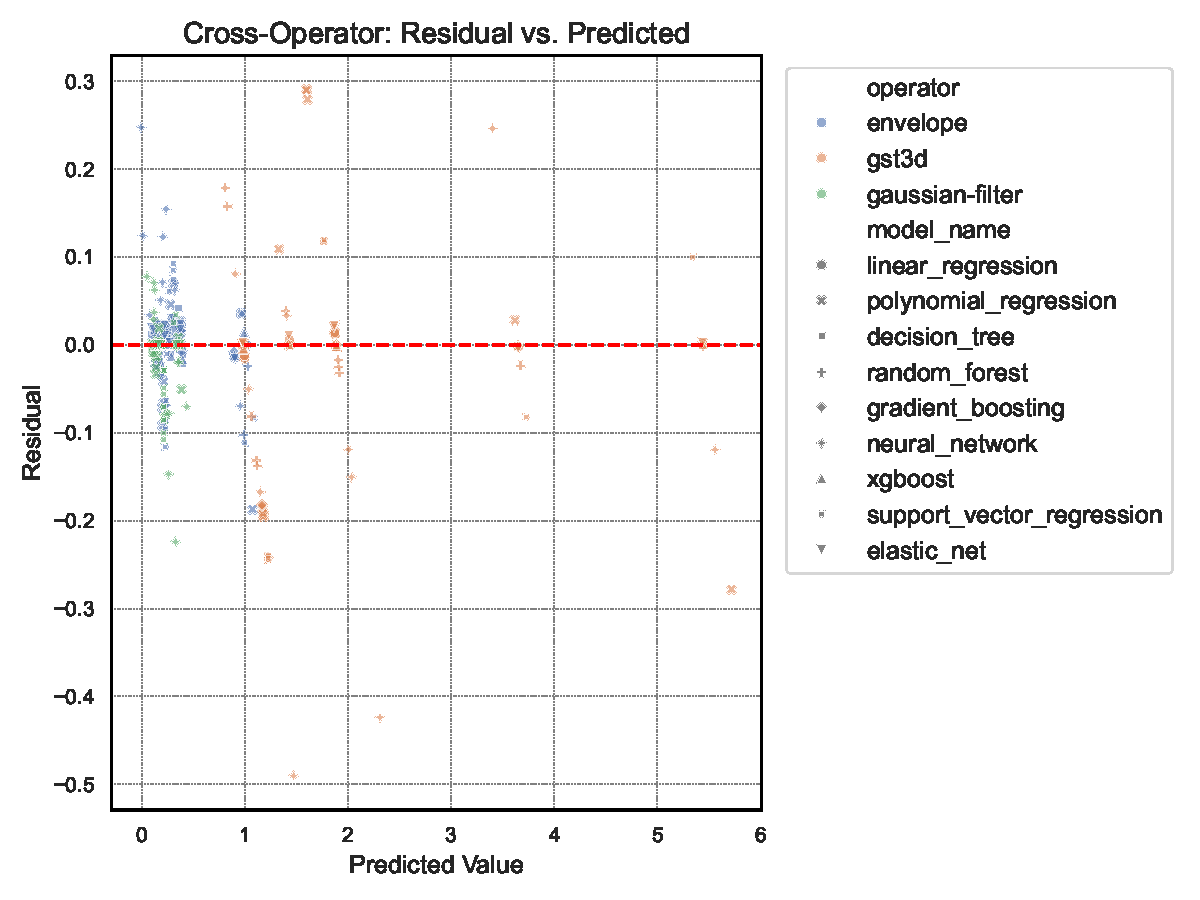
\includegraphics[width=\textwidth]{assets/images/05/residual_vs_predicted}
        \caption{Residual vs.\ predicted values for all operators and models.
            Most models yield low residuals across a wide range of predicted values.
            The \ac{GST3D}–Neural Network pairing stands out for higher errors.
            \EB{Adicione a unidade de medida nos rótulos dos eixos: p.ex.: Residual (GB?) e Predicted Value (GB?)}
        }
    \end{subfigure}
    \hfill
    \begin{subfigure}[t]{0.49\textwidth}
        \centering
        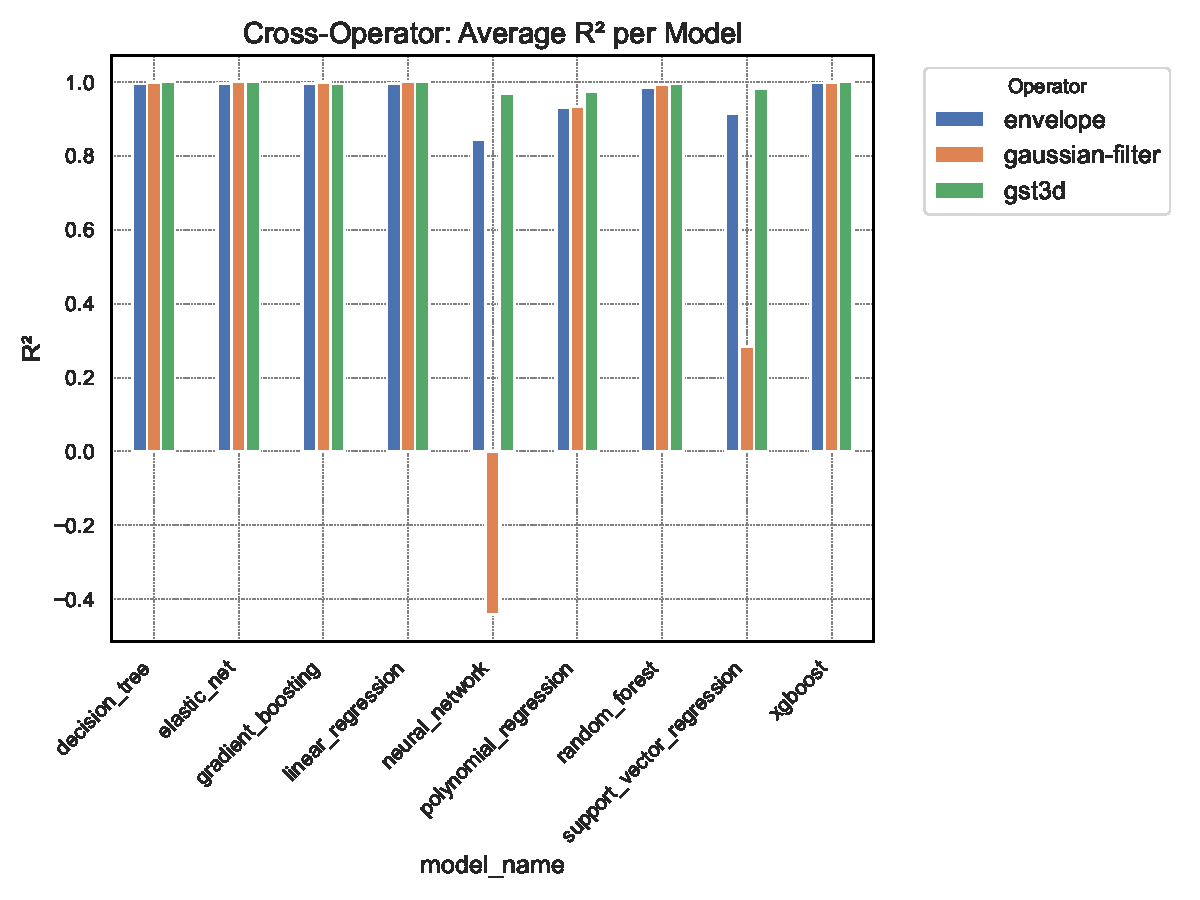
\includegraphics[width=\textwidth]{assets/images/05/cross_model_r2_bar}
        \caption{$R^2$ scores for each model and operator.
        Linear Regression, XGBoost, and Elastic Net perform consistently well.
        The Neural Network underperforms for \ac{GST3D}.}
    \end{subfigure}
    \caption{Overview of cross-model results: (a) residual-versus-predicted scatter plots and (b) $R^2$ bar chart.
        Simpler or regularized linear methods often yield the most stable fits.
        \EB{As fontes destes gráficos estão muito pequenas. Acho que ficaria melhor separar em dois gráficos. Não tenho certeza, mas talvez os dados do gráfico (b) fiquem melhor em uma tabela.}
        \label{fig:residual_vs_predicted_and_r2_bar}
    }
\end{figure*}

Table~\ref{tab:performance_summary} summarizes the main metrics for each operator, aggregated over the nine models.
These data are distilled from the experiment’s \texttt{model\_metrics.csv} files (Envelope, \ac{GST3D}, Gaussian Filter).
The best \EBC{“score”}{definir esta métrica} values for Envelope, \ac{GST3D}, and Gaussian Filter are $2.579$, $2.970$, and $2.904$, respectively.
Gradient Boosting tops Envelope, Decision Tree leads \ac{GST3D}, and Linear Regression narrowly surpasses Elastic Net for the Gaussian Filter.

\begin{table}[htbp]
    \centering
    \begin{tabular}{lccc}
        \hline
        \textbf{Operator} & \textbf{Best Model} & \textbf{Best Score} & \textbf{Note}                    \\
        \hline
        Envelope          & Gradient Boosting   & 2.579               & Consistently low RMSE            \\
        \ac{GST3D}        & Decision Tree       & 2.970               & Highest $R^2$, minimal residuals \\
        Gaussian Filter   & Linear Regression   & 2.904               & Ties closely with Elastic Net    \\
        \hline
    \end{tabular}
    \caption{Summary of top-performing models and their best “score” metric across operators.}
    \label{tab:performance_summary}
\end{table}

\subsection{Operator-Specific Model Scores}
\label{subsec:operator-specific-model-scores}

Figures~\ref{fig:score_by_model_operators} and~\ref{fig:best_model_per_operator} break down model \EBC{scores}{definir esta métrica} per operator and highlight the winning algorithm in each category.
The minor differences among the leading models (Gradient Boosting, XGBoost, Decision Tree, and Linear/Elastic Net) suggest that seismic memory usage is comparatively straightforward to learn, likely due to the near-linear volume relationship observed in Section~\ref{sec:pmc-results-memory-and-execution-time-profiling}.

\begin{figure*}[htbp]
    \centering
    \begin{subfigure}[t]{0.32\textwidth}
        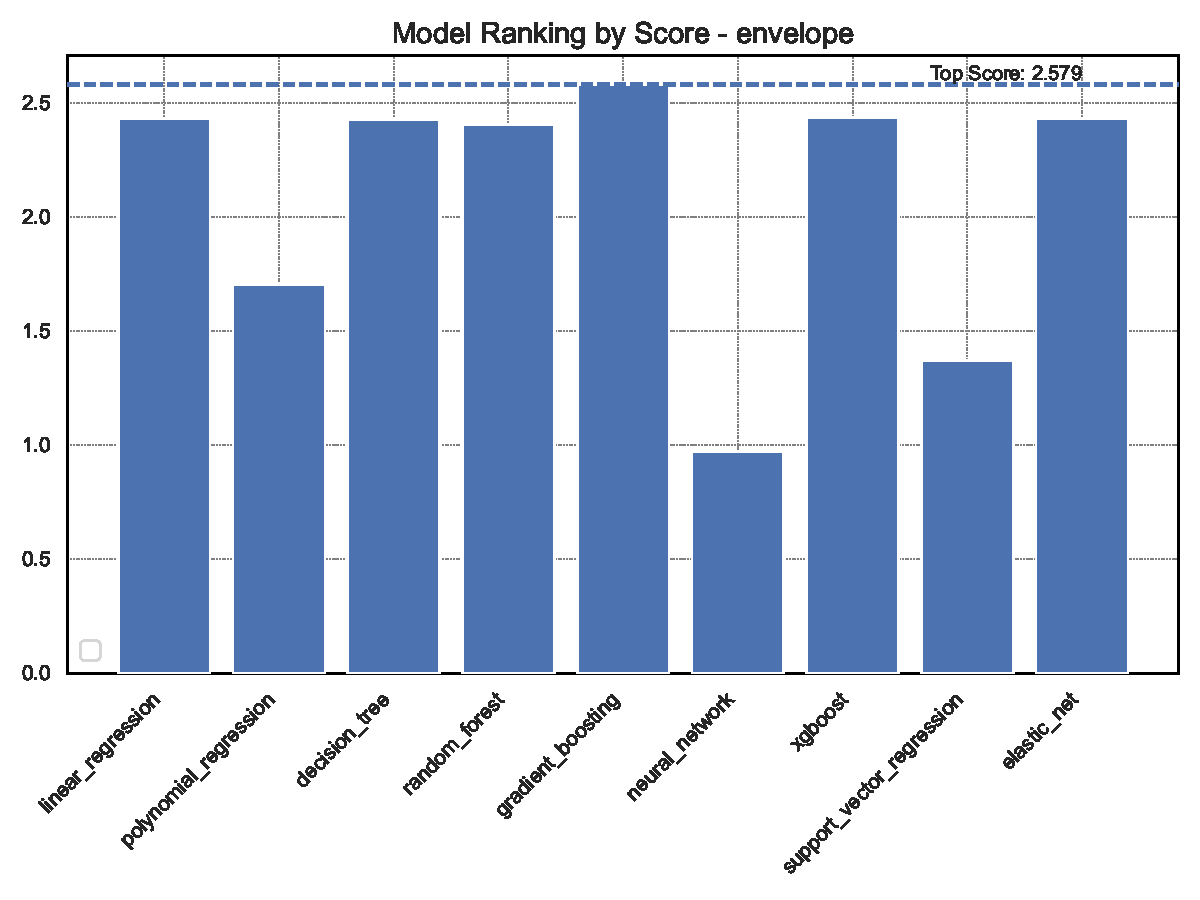
\includegraphics[width=\textwidth]{assets/images/05/score_by_model_envelope}
        \caption{Envelope}
    \end{subfigure}
    \hfill
    \begin{subfigure}[t]{0.32\textwidth}
        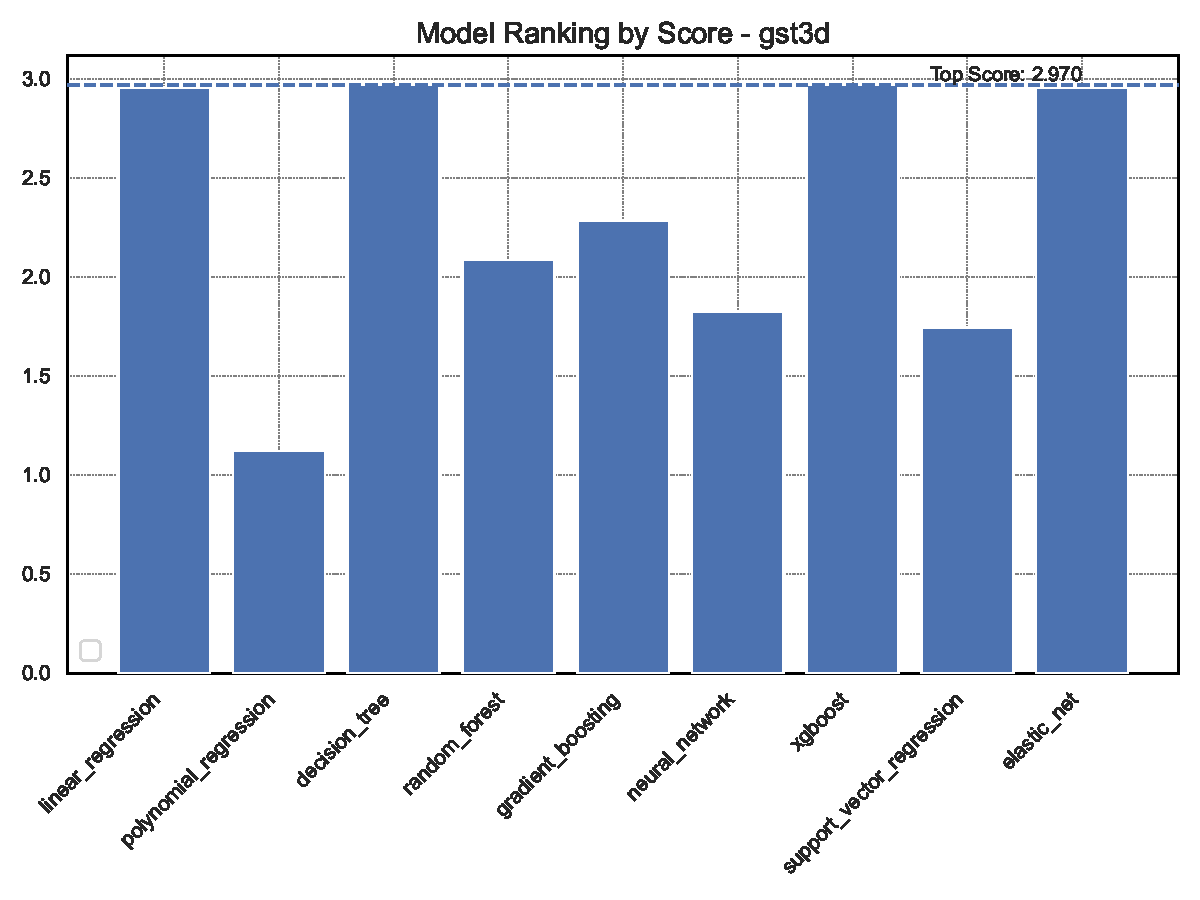
\includegraphics[width=\textwidth]{assets/images/05/score_by_model_gst3d}
        \caption{\ac{GST3D}}
    \end{subfigure}
    \hfill
    \begin{subfigure}[t]{0.32\textwidth}
        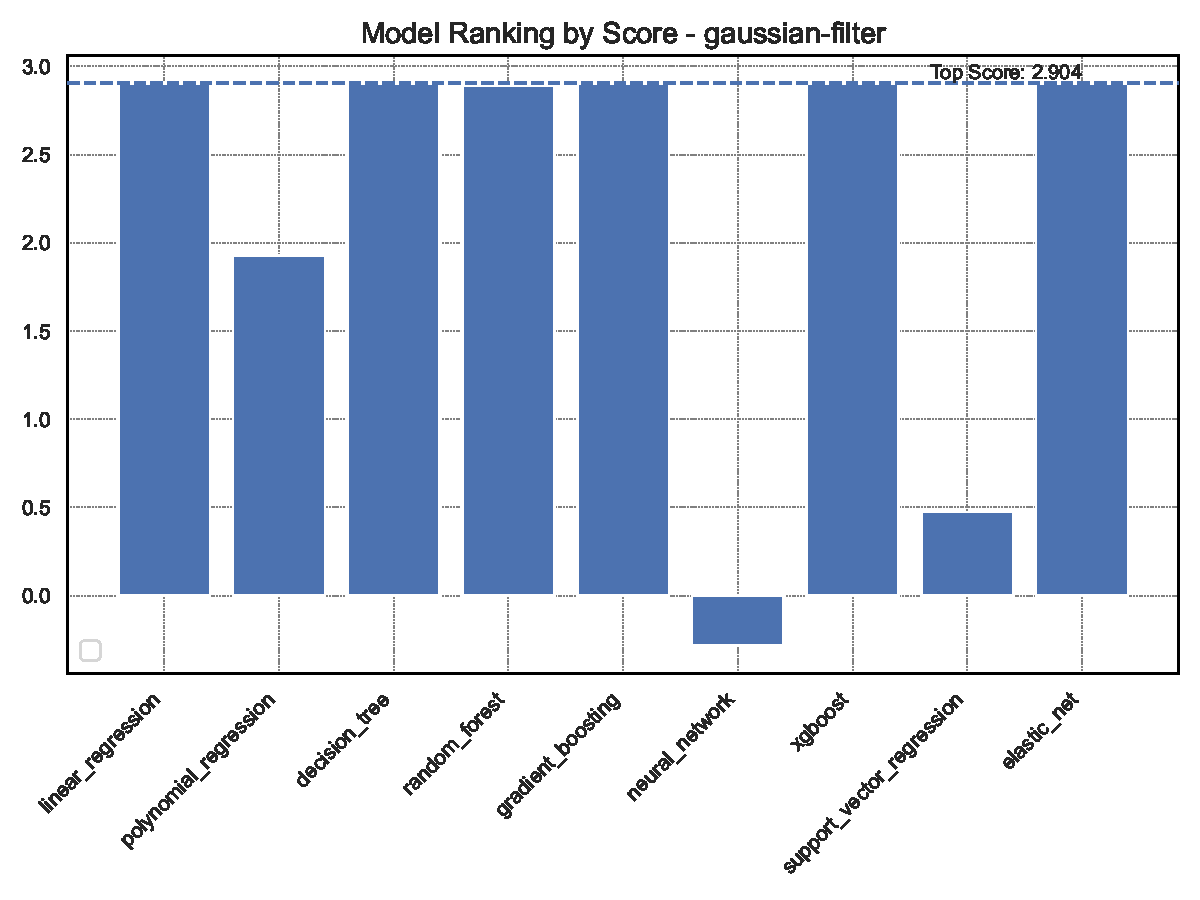
\includegraphics[width=\textwidth]{assets/images/05/score_by_model_gaussian-filter}
        \caption{Gaussian Filter}
    \end{subfigure}
    \caption{\EBC{Scores by model for each operator}{definir a métrica score}.
        A higher score indicates stronger overall performance.
        Multiple models cluster near the top for all three operators, highlighting the relative ease of predicting memory usage from linear shape parameters.
        \label{fig:score_by_model_operators}
    }
\end{figure*}

\begin{figure}[htbp]
    \centering
    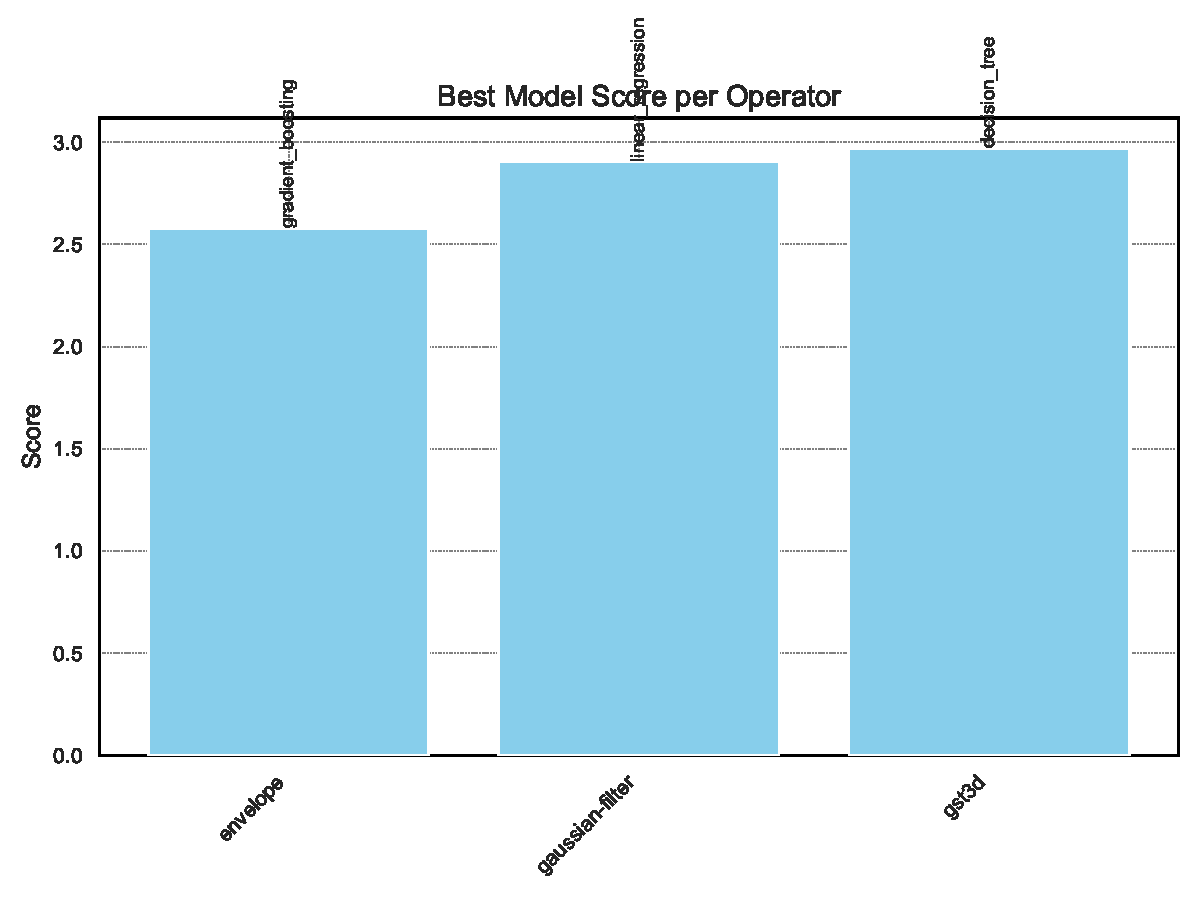
\includegraphics[width=0.6\textwidth]{assets/images/05/best_model_per_operator}
    \caption{Best model per operator by score: Gradient Boosting (Envelope), Decision Tree (\ac{GST3D}), and Linear Regression (Gaussian Filter).
        \EB{Senti falta da definição da métrica "Score"}
        \label{fig:best_model_per_operator}
    }
\end{figure}

\subsection{Accuracy and RMSE Analysis}
\label{subsec:accuracy-and-rmse-analysis}

\EBC{Como você definiu/calculou acurácia?}

Figure~\ref{fig:accuracy_rmse_envelope} illustrates accuracy versus \ac{RMSE} for each model under Envelope, \ac{GST3D}, and Gaussian Filter.
An ideal model would appear near the top-left corner (high accuracy, low \ac{RMSE}).
Polynomial Regression and the Neural Network exhibit relatively higher \ac{RMSE} in \ac{GST3D}, reinforcing the patterns already noted in the residual plots and $R^2$ bars.

\begin{figure*}[htbp]
    \centering
    \begin{subfigure}[t]{0.32\textwidth}
        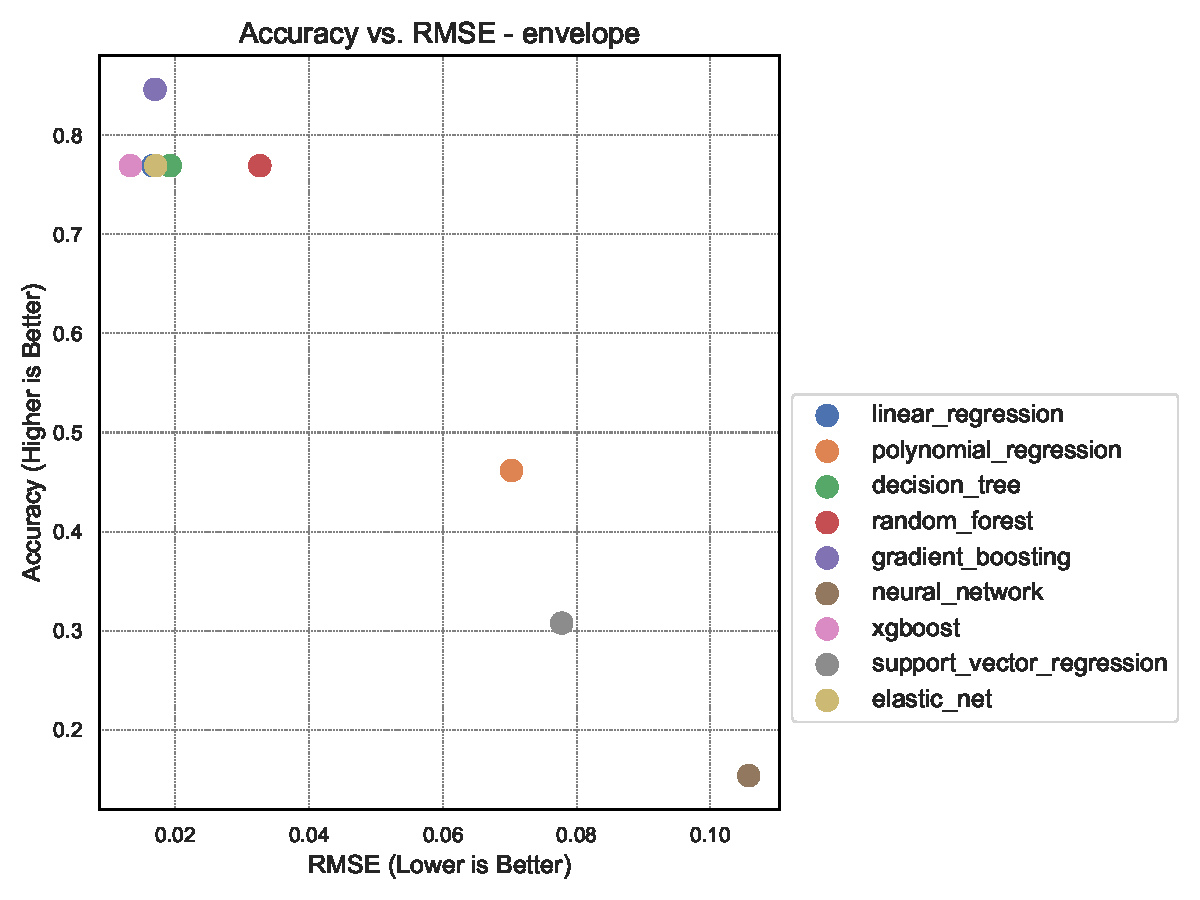
\includegraphics[width=\textwidth]{assets/images/05/accuracy_by_rmse_per_model_envelope}
        \caption{Envelope}
    \end{subfigure}
    \hfill
    \begin{subfigure}[t]{0.32\textwidth}
        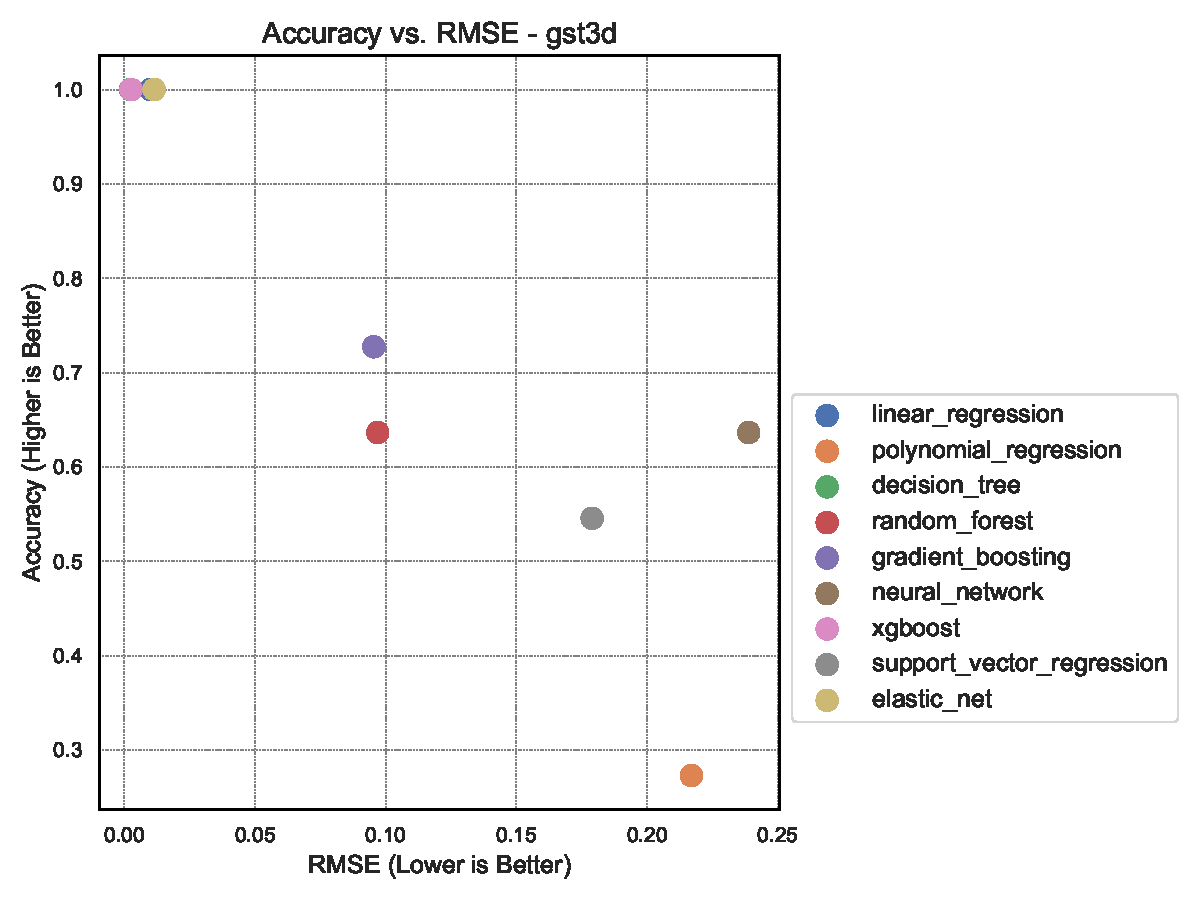
\includegraphics[width=\textwidth]{assets/images/05/accuracy_by_rmse_per_model_gst3d}
        \caption{\ac{GST3D}}
    \end{subfigure}
    \hfill
    \begin{subfigure}[t]{0.32\textwidth}
        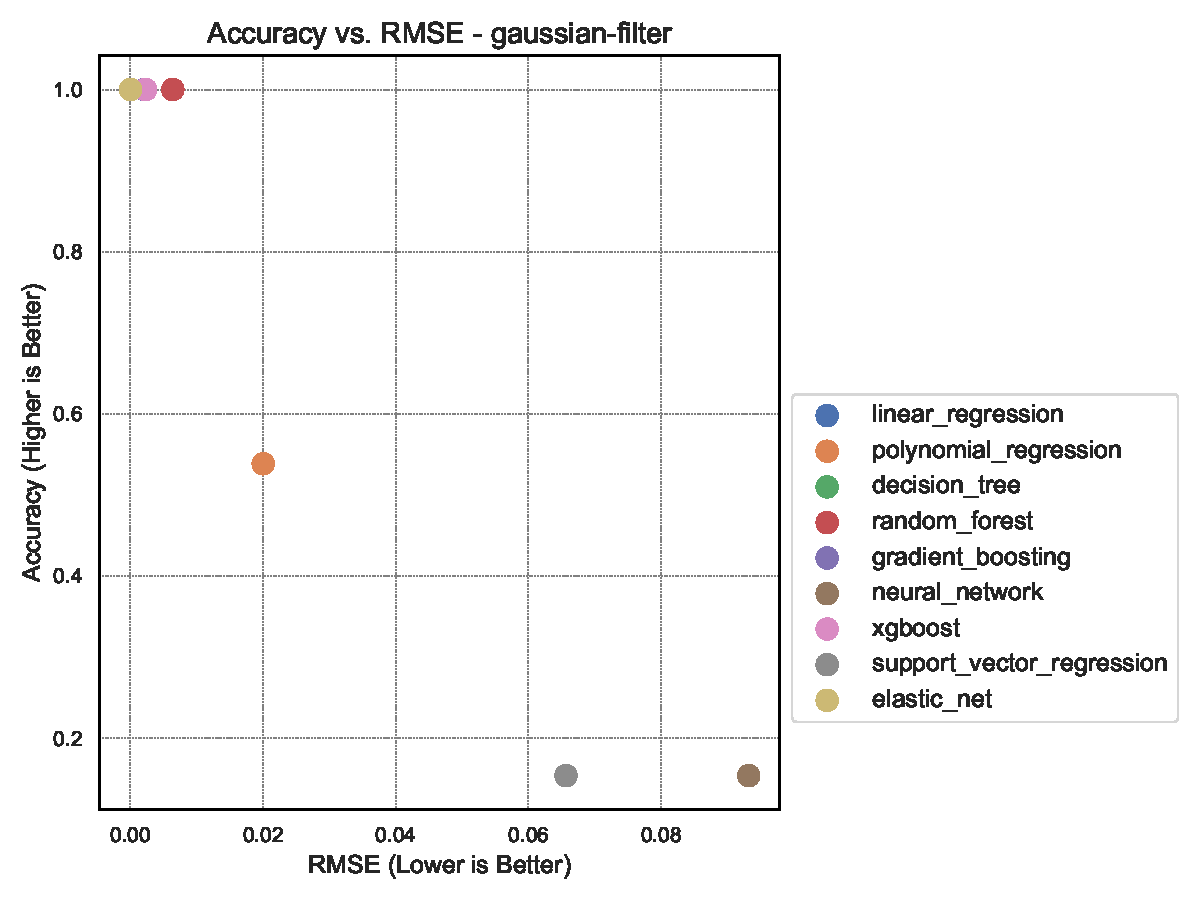
\includegraphics[width=\textwidth]{assets/images/05/accuracy_by_rmse_per_model_gaussian-filter}
        \caption{Gaussian Filter}
    \end{subfigure}
    \caption{Accuracy vs.\ \ac{RMSE} per model and operator.
        Most methods attain near-perfect metrics for Envelope and Gaussian Filter.
        \ac{GST3D} displays higher \ac{RMSE} for polynomial and Neural Network approaches.
        \EB{Acho que ficaria melhor compartilhando a legenda - com apenas uma legenda.}
    }
    \label{fig:accuracy_rmse_envelope}
\end{figure*}

\subsection{Actual vs.\ Predicted Plots and Residual Distributions}
\label{subsec:actual-vs-predicted-and-residual-distributions}

Figure~\ref{fig:actual_vs_predicted} compare actual and predicted memory usage for each operator and model.
The best fits produce data points that lie close to the diagonal line, implying minimal error.
Linear Regression, XGBoost, and Elastic Net nearly overlap with the diagonal for Envelope and Gaussian Filter.
Decision Tree does likewise for \ac{GST3D}.

\begin{figure*}[htbp]
    \centering
    \begin{subfigure}[t]{0.32\textwidth}
        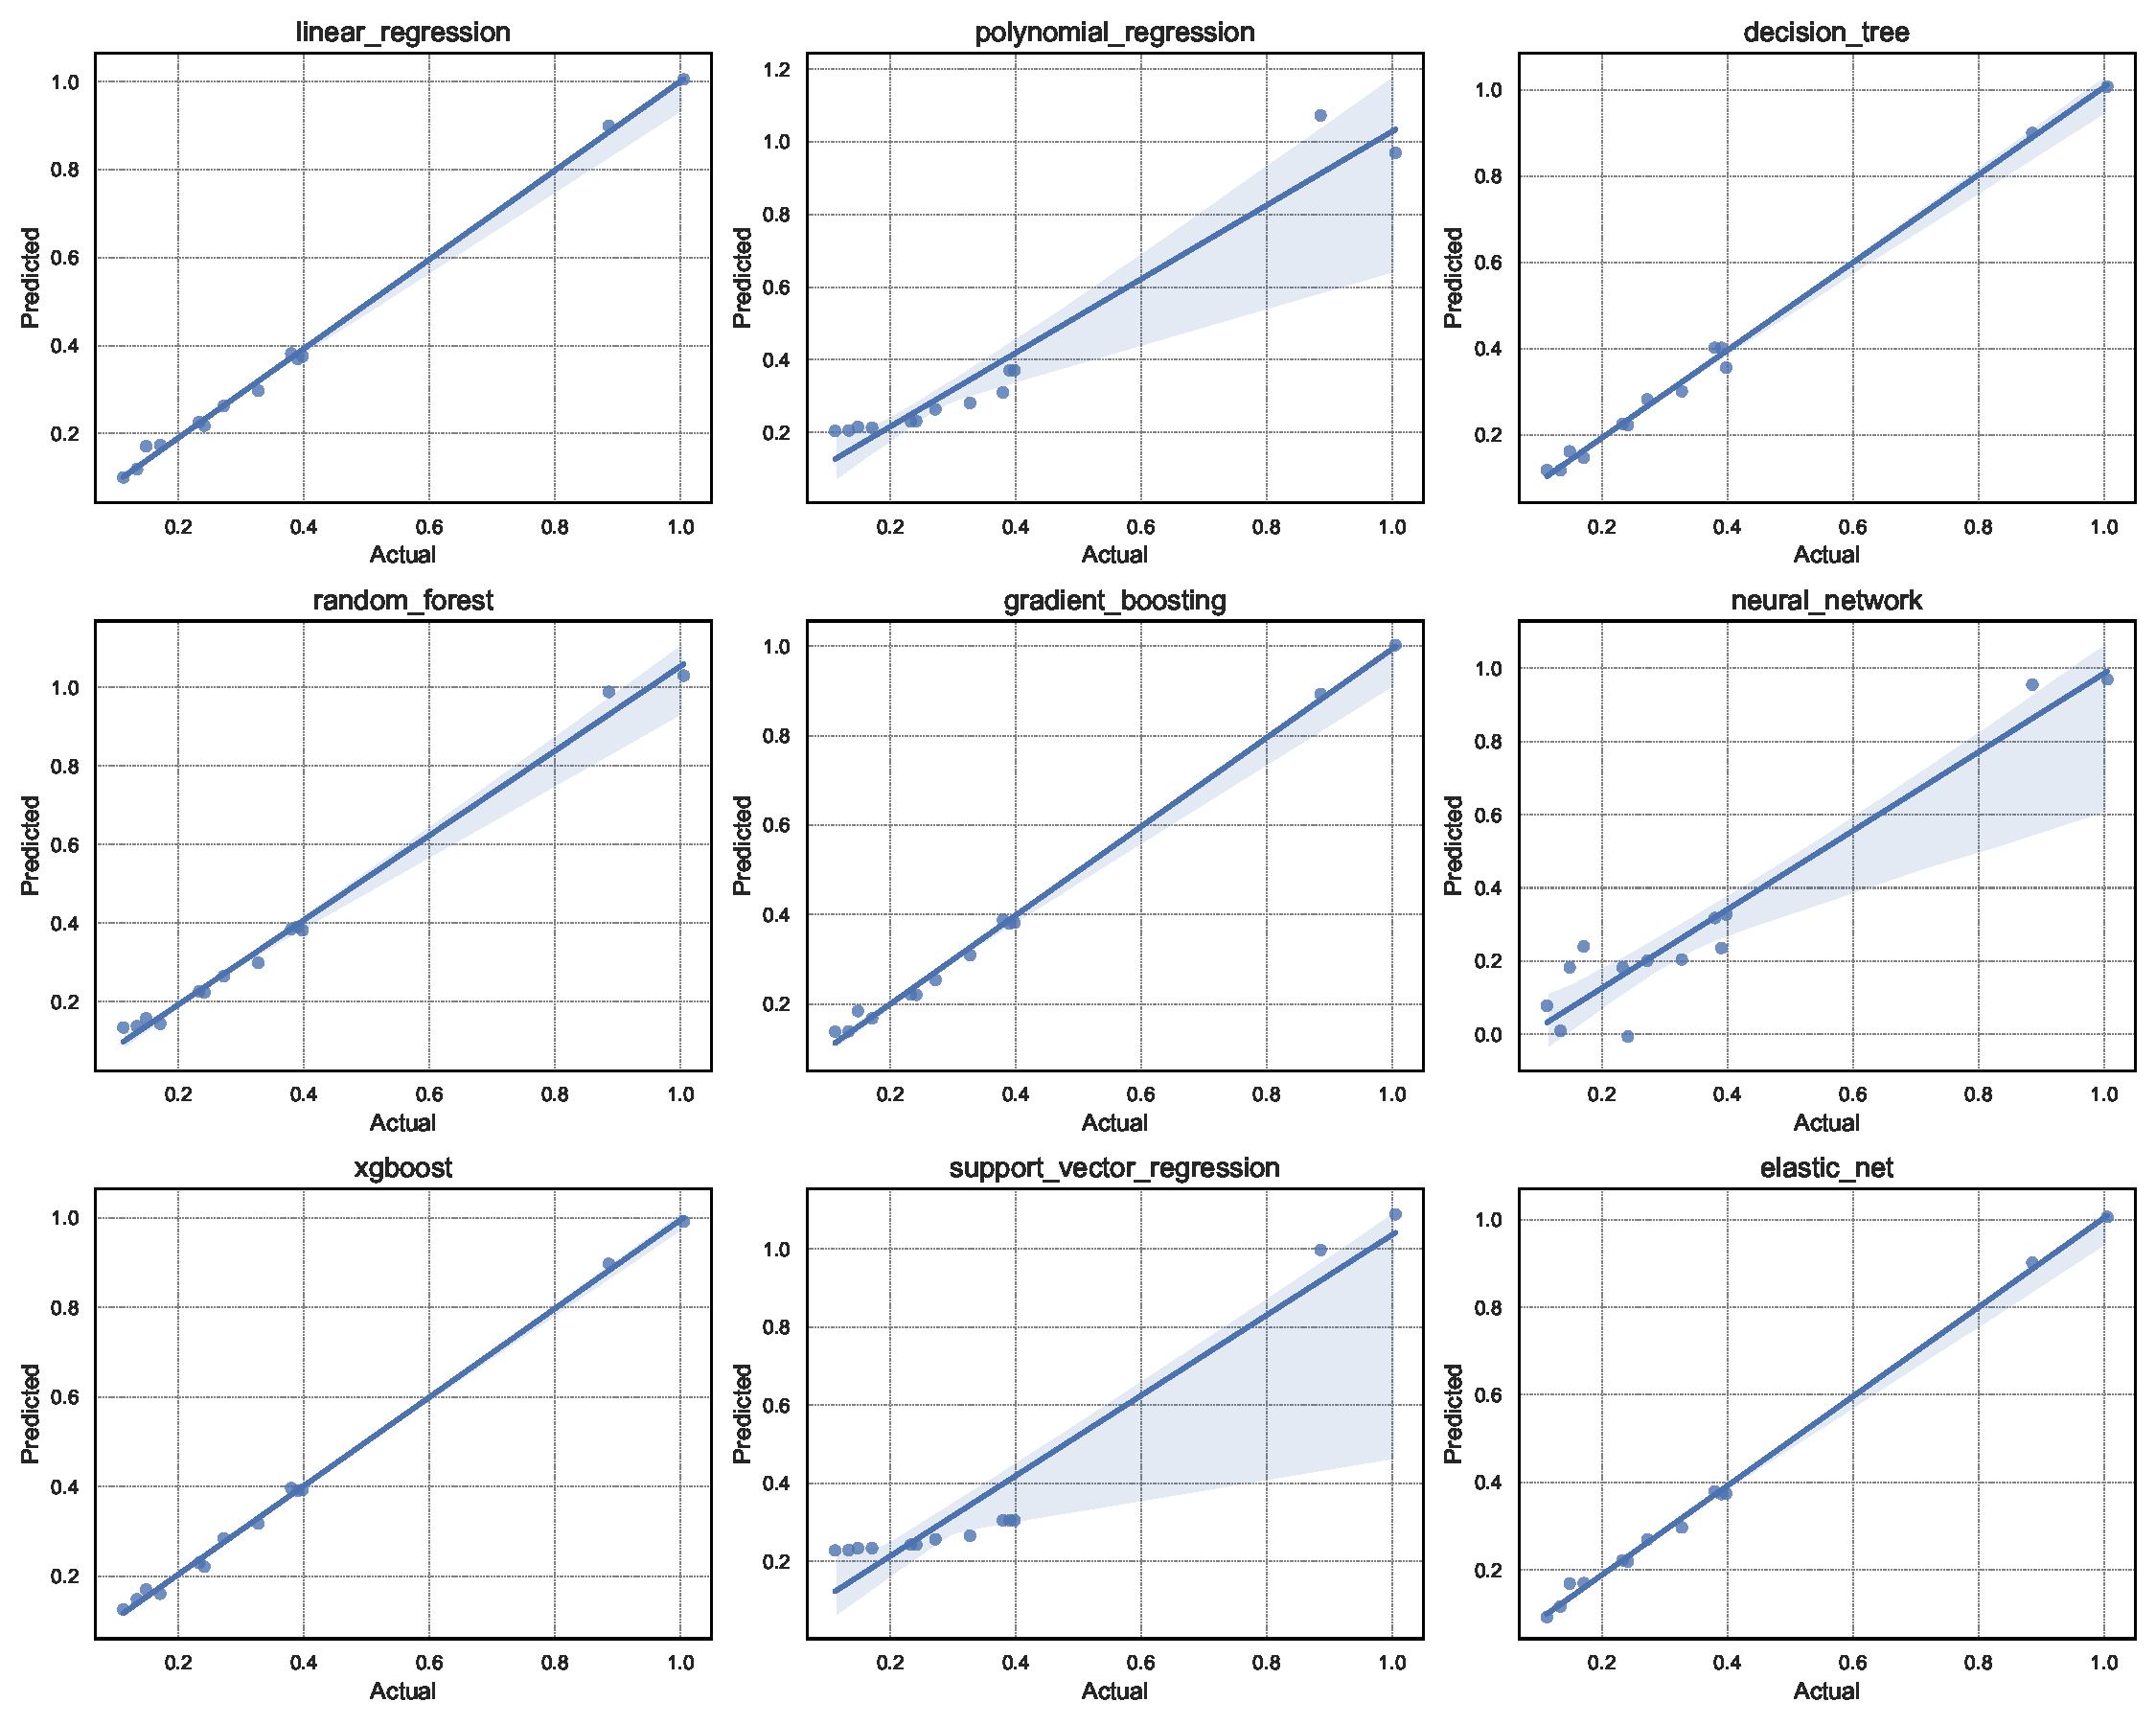
\includegraphics[width=\textwidth]{assets/images/05/actual_vs_predicted_by_model_envelope}
        \caption{Envelope}
    \end{subfigure}
    \hfill
    \begin{subfigure}[t]{0.32\textwidth}
        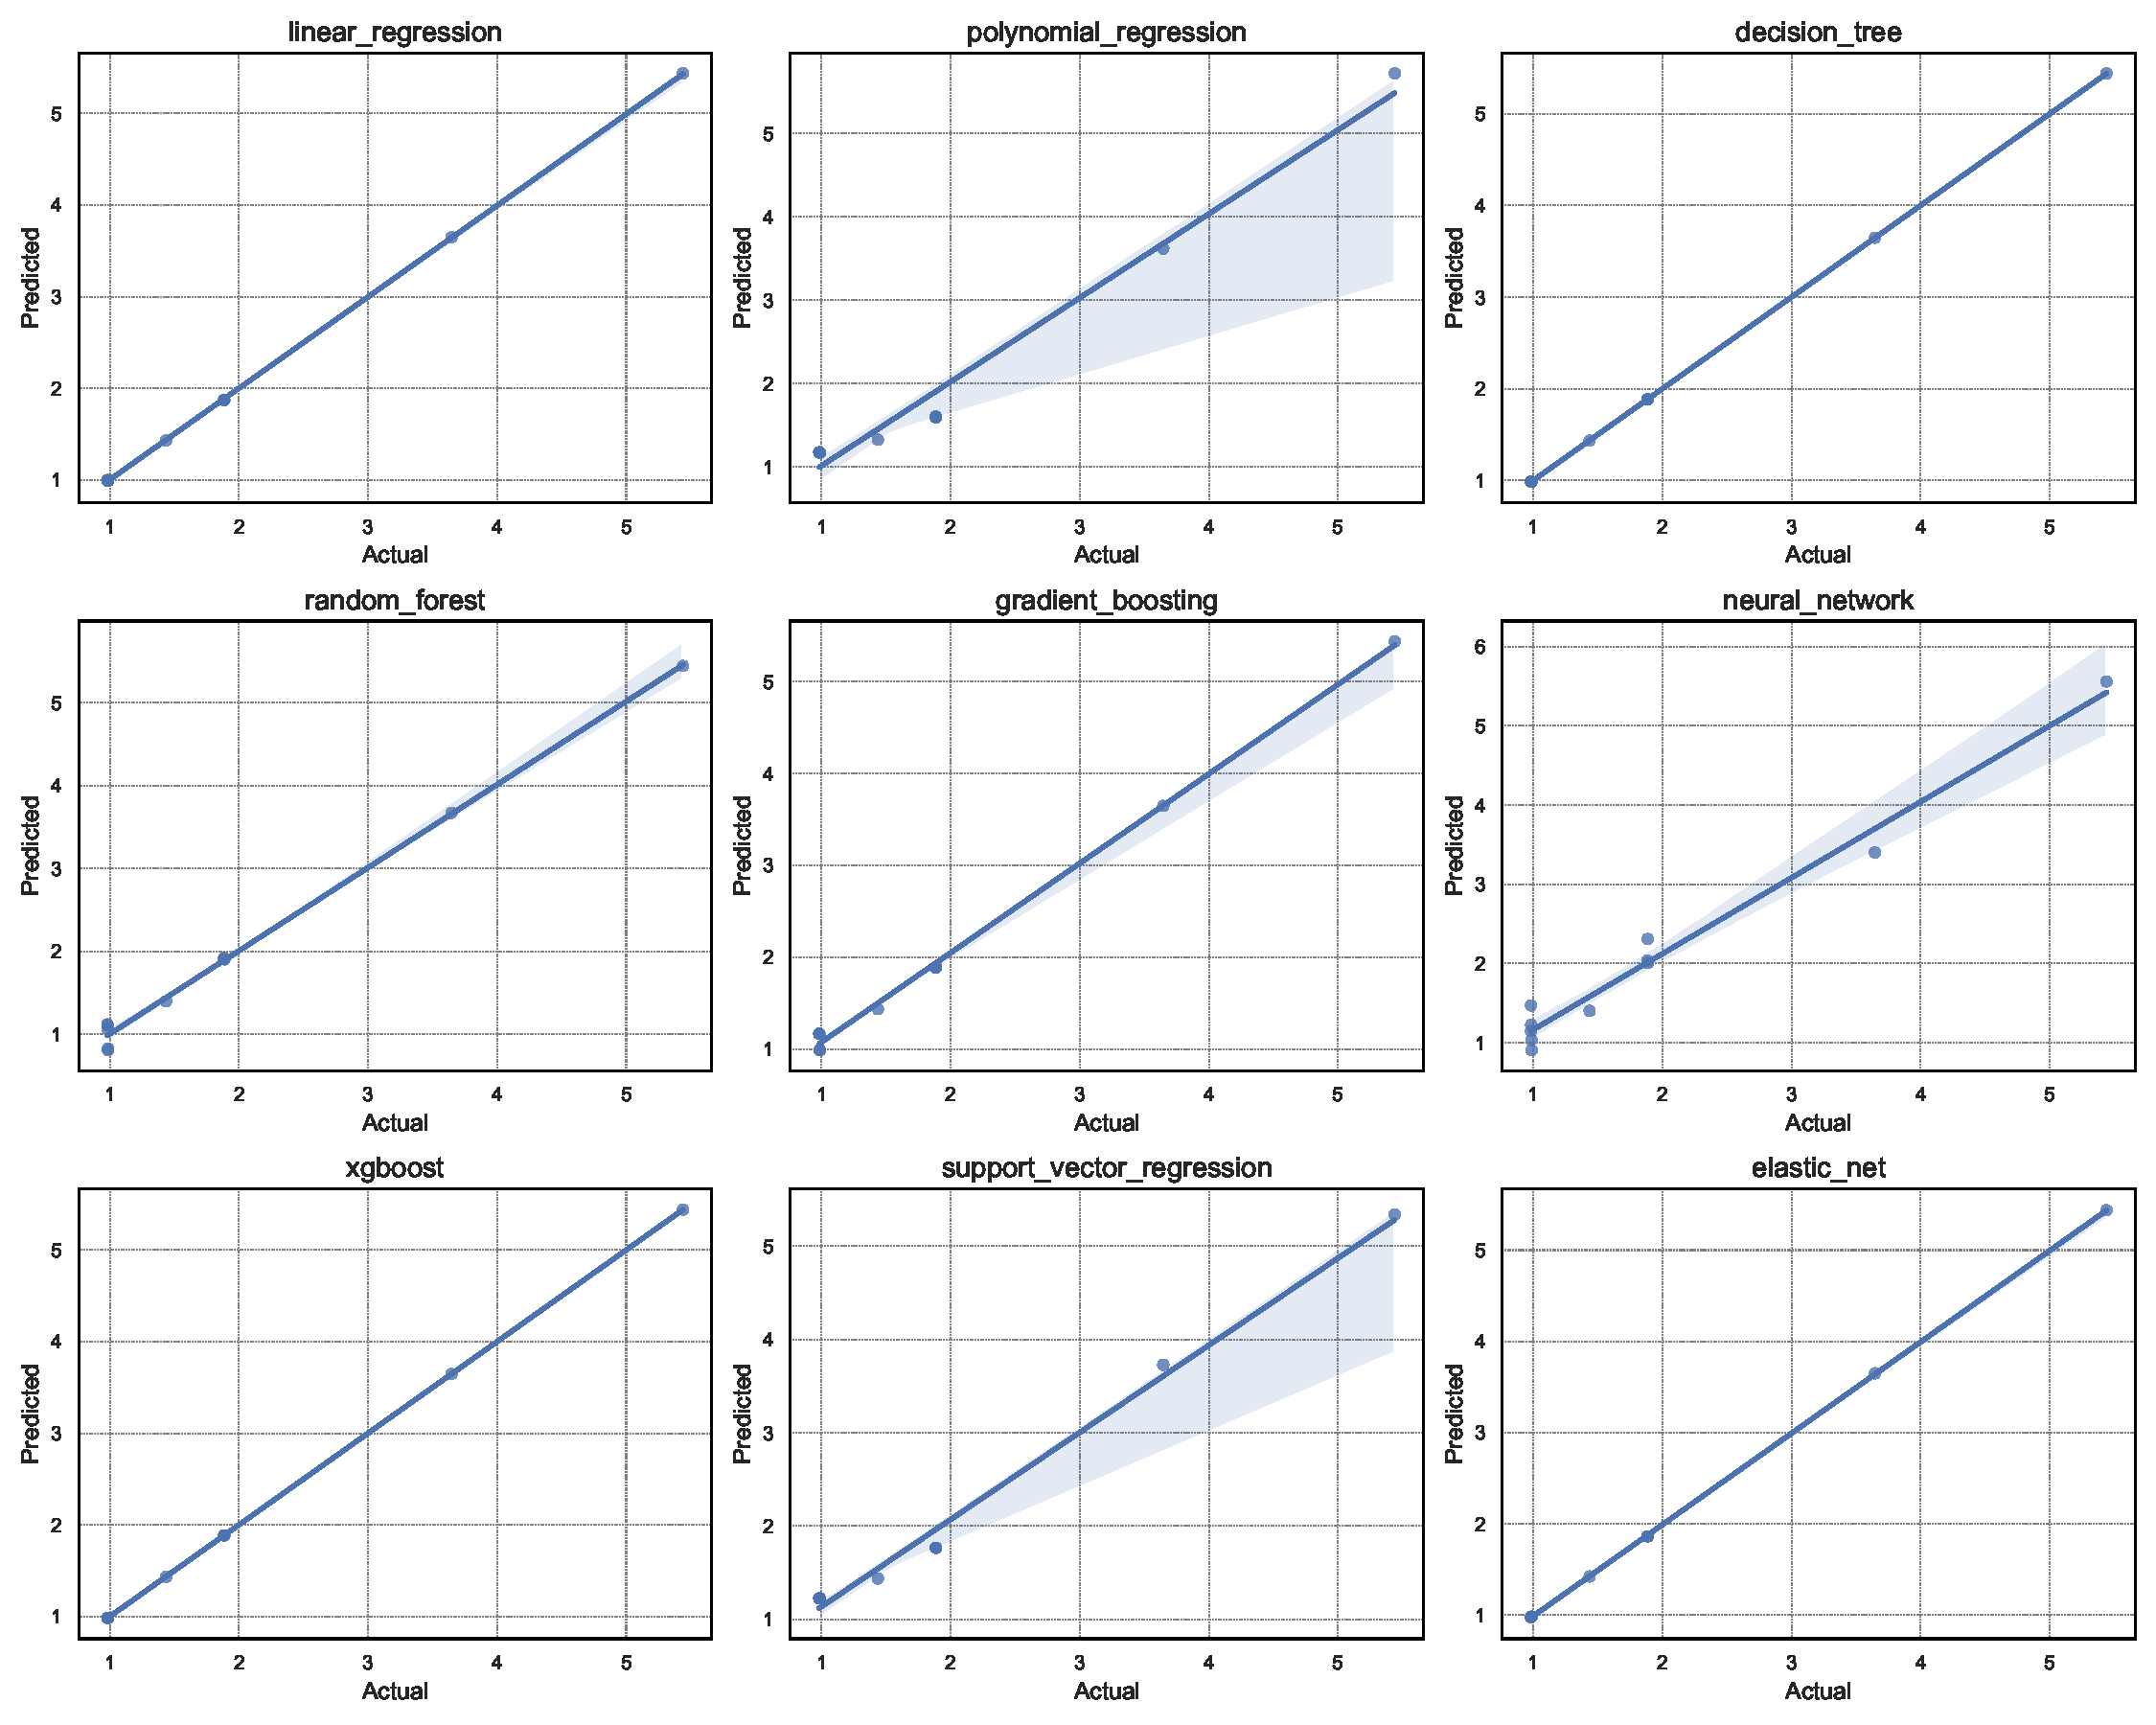
\includegraphics[width=\textwidth]{assets/images/05/actual_vs_predicted_by_model_gst3d}
        \caption{\ac{GST3D}}
    \end{subfigure}
    \hfill
    \begin{subfigure}[t]{0.32\textwidth}
        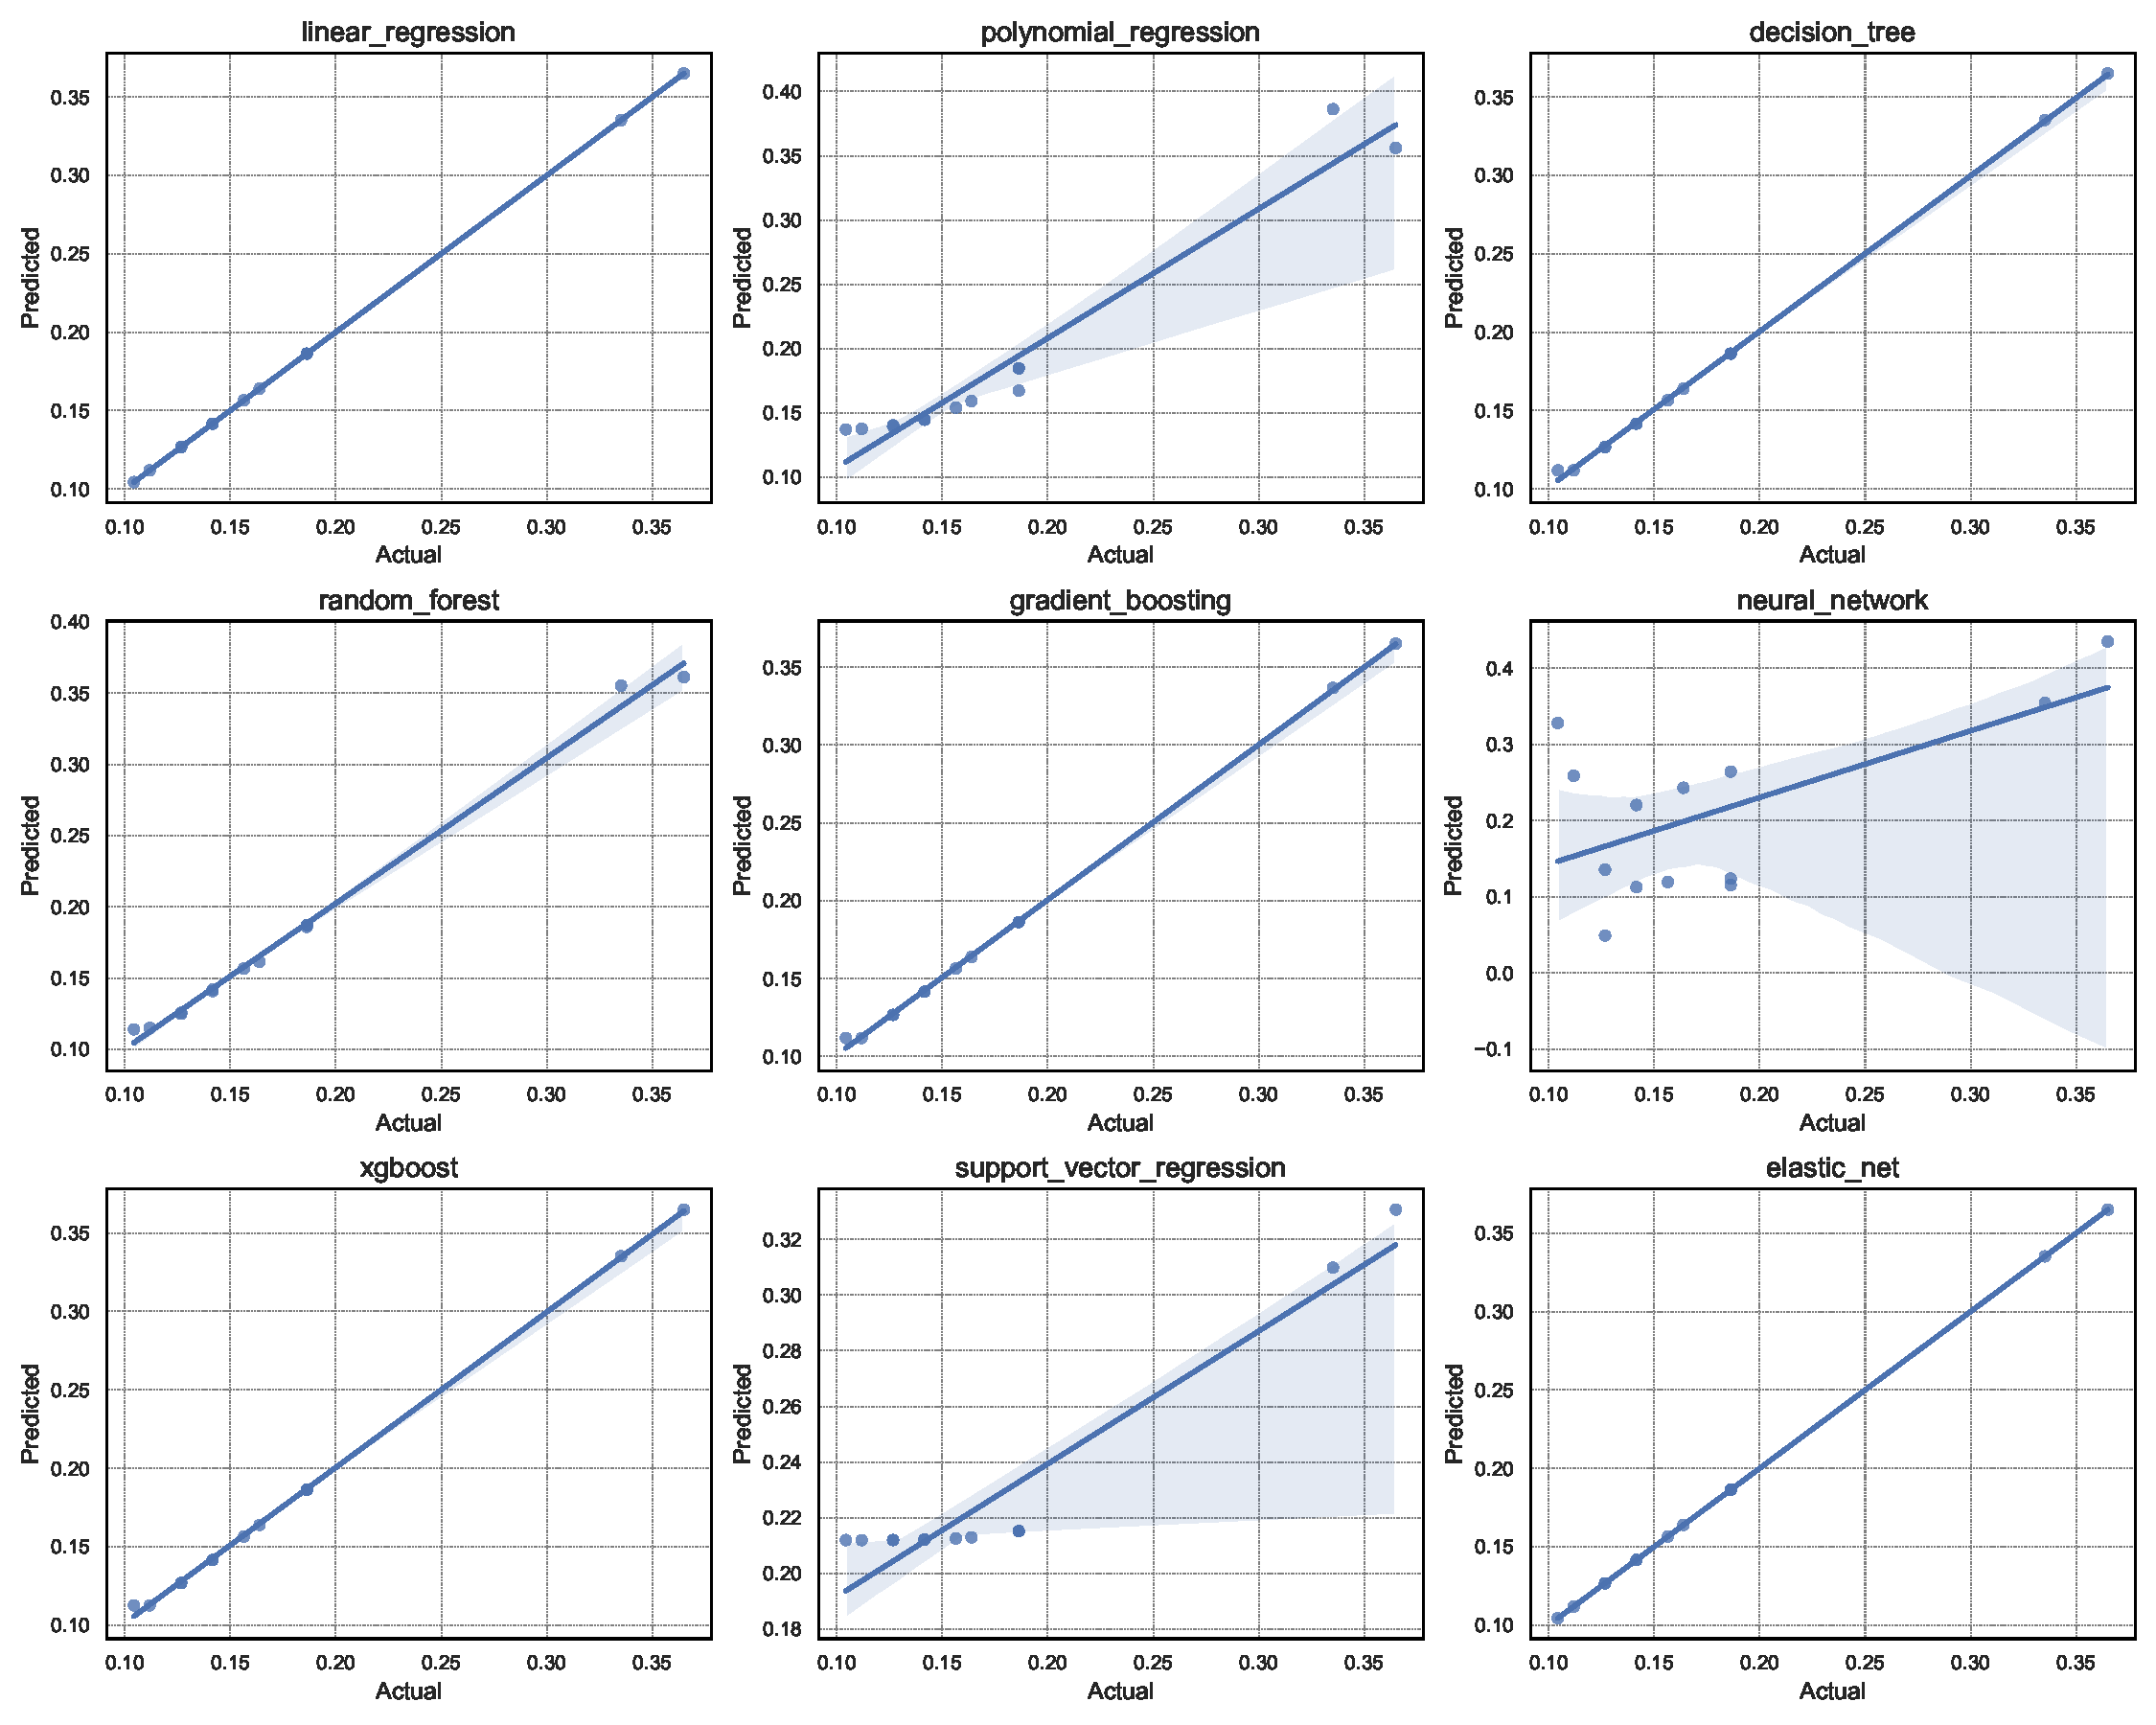
\includegraphics[width=\textwidth]{assets/images/05/actual_vs_predicted_by_model_gaussian-filter}
        \caption{Gaussian Filter}
    \end{subfigure}
    \caption{Actual vs.\ predicted memory usage for each operator.
    A nearly diagonal trend indicates that the model approximates the real consumption.
    The Neural Network struggles slightly more for \ac{GST3D}, but most others fit well.}
    \label{fig:actual_vs_predicted}
\end{figure*}

Figures~\ref{fig:residual_qq_plots} show residual \ac{QQ} plots.
Points that track the diagonal suggest normally distributed residuals, indicating no major systematic bias.
Gradient Boosting, Random Forest, and XGBoost residuals remain closer to this line than Neural Network or Polynomial Regression, which exhibit heavier tails or skew.
However, none of the models produce perfectly normal residuals, which is common in real-world \ac{HPC} \EBC{data.}{Adicionar uma referência para dar suporte a esta afirmação}

\begin{figure*}[htbp]
    \centering
    \begin{subfigure}[t]{0.32\textwidth}
        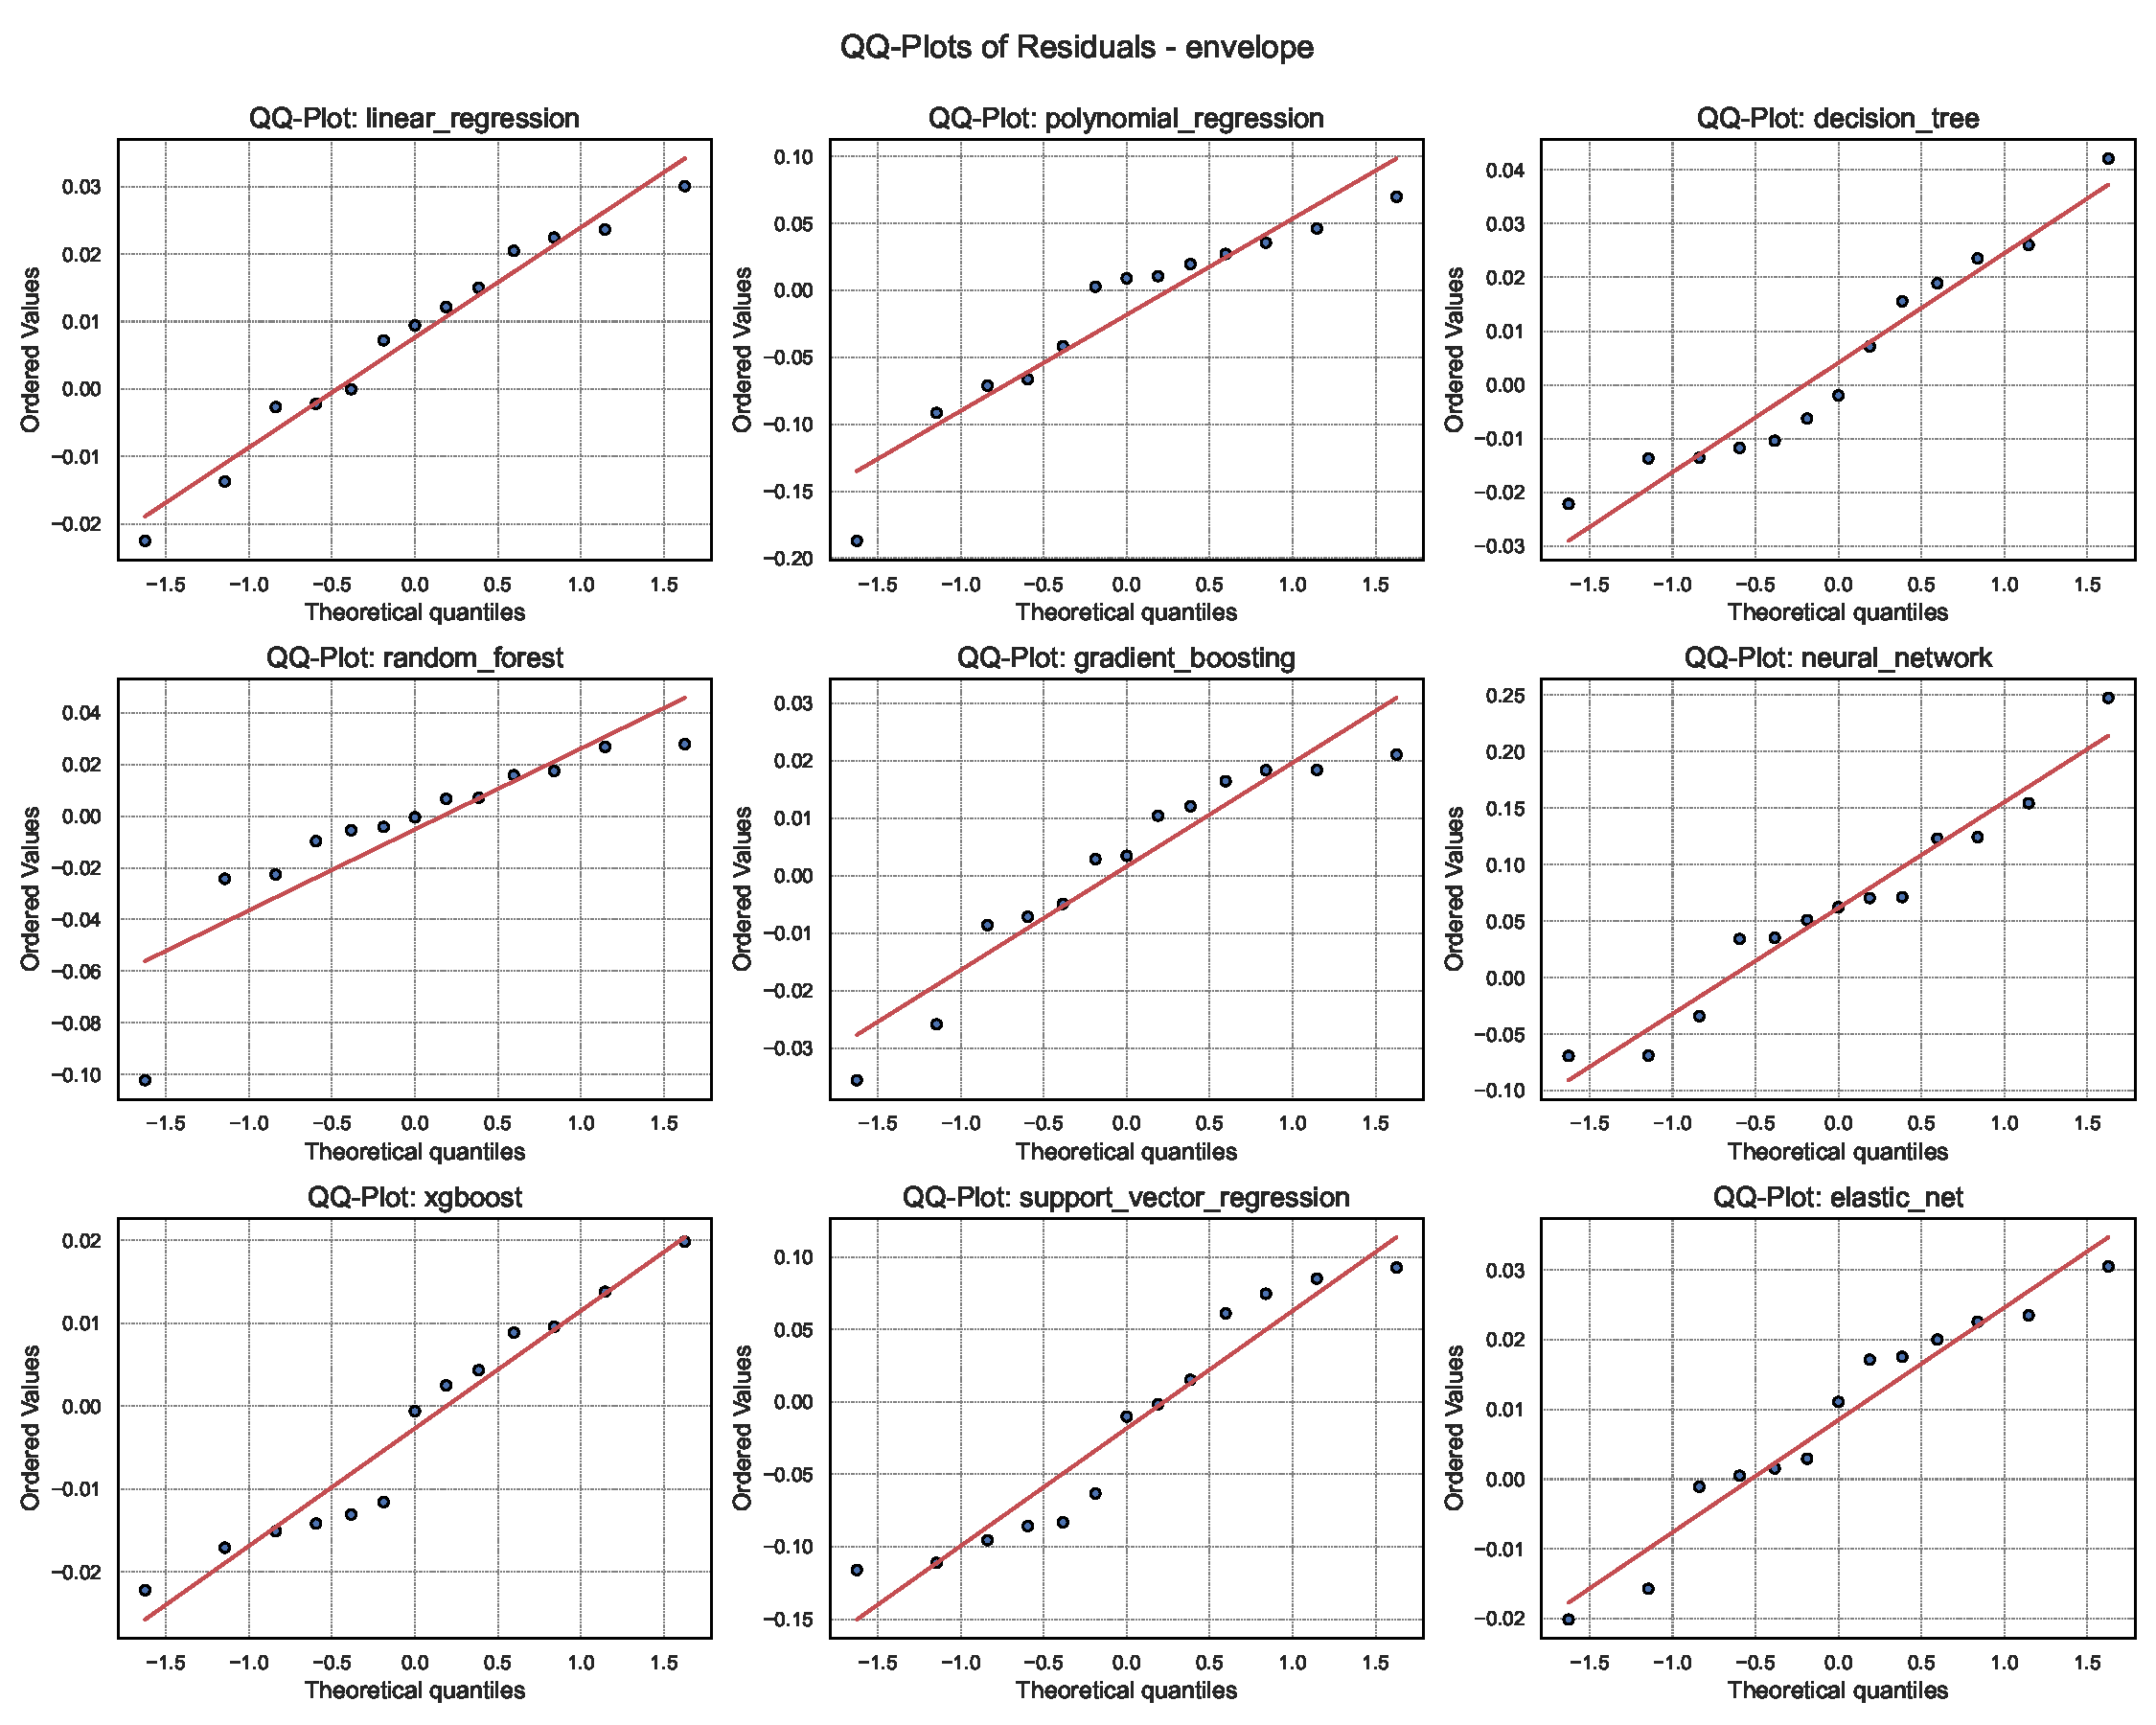
\includegraphics[width=\textwidth]{assets/images/05/residual_qq_plots_envelope}
        \caption{Envelope}
    \end{subfigure}
    \hfill
    \begin{subfigure}[t]{0.32\textwidth}
        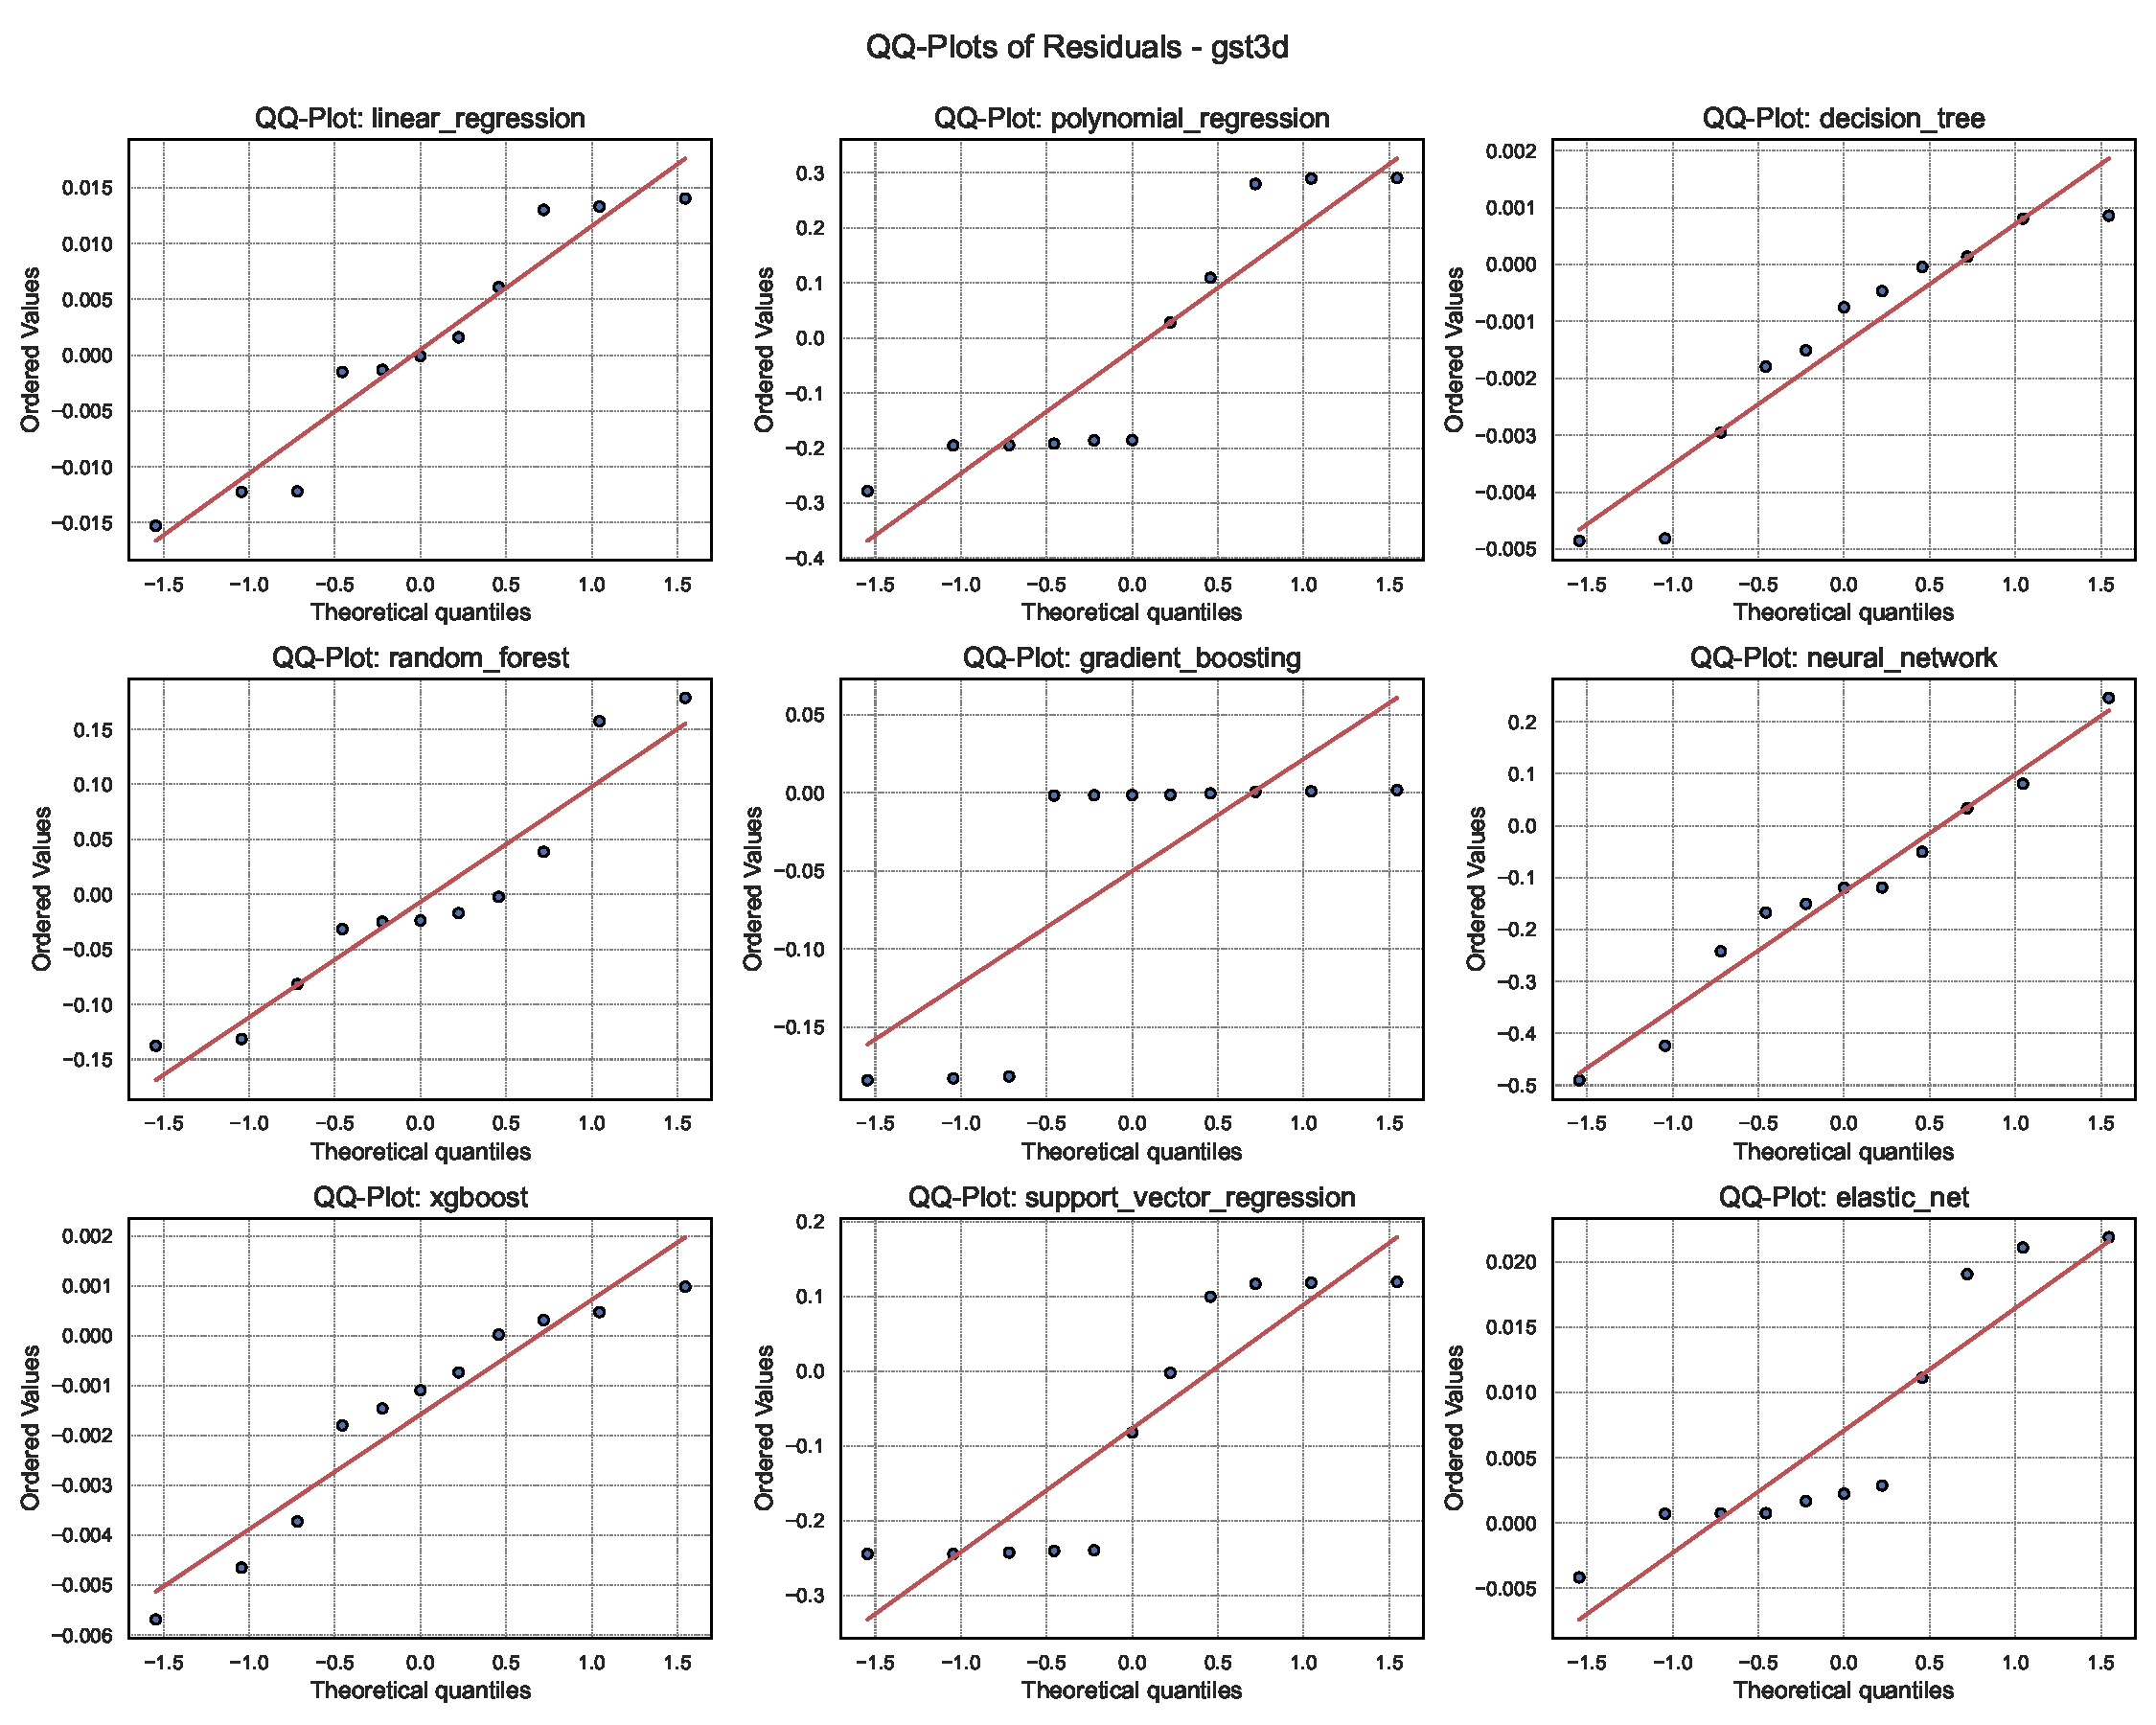
\includegraphics[width=\textwidth]{assets/images/05/residual_qq_plots_gst3d}
        \caption{\ac{GST3D}}
    \end{subfigure}
    \hfill
    \begin{subfigure}[t]{0.32\textwidth}
        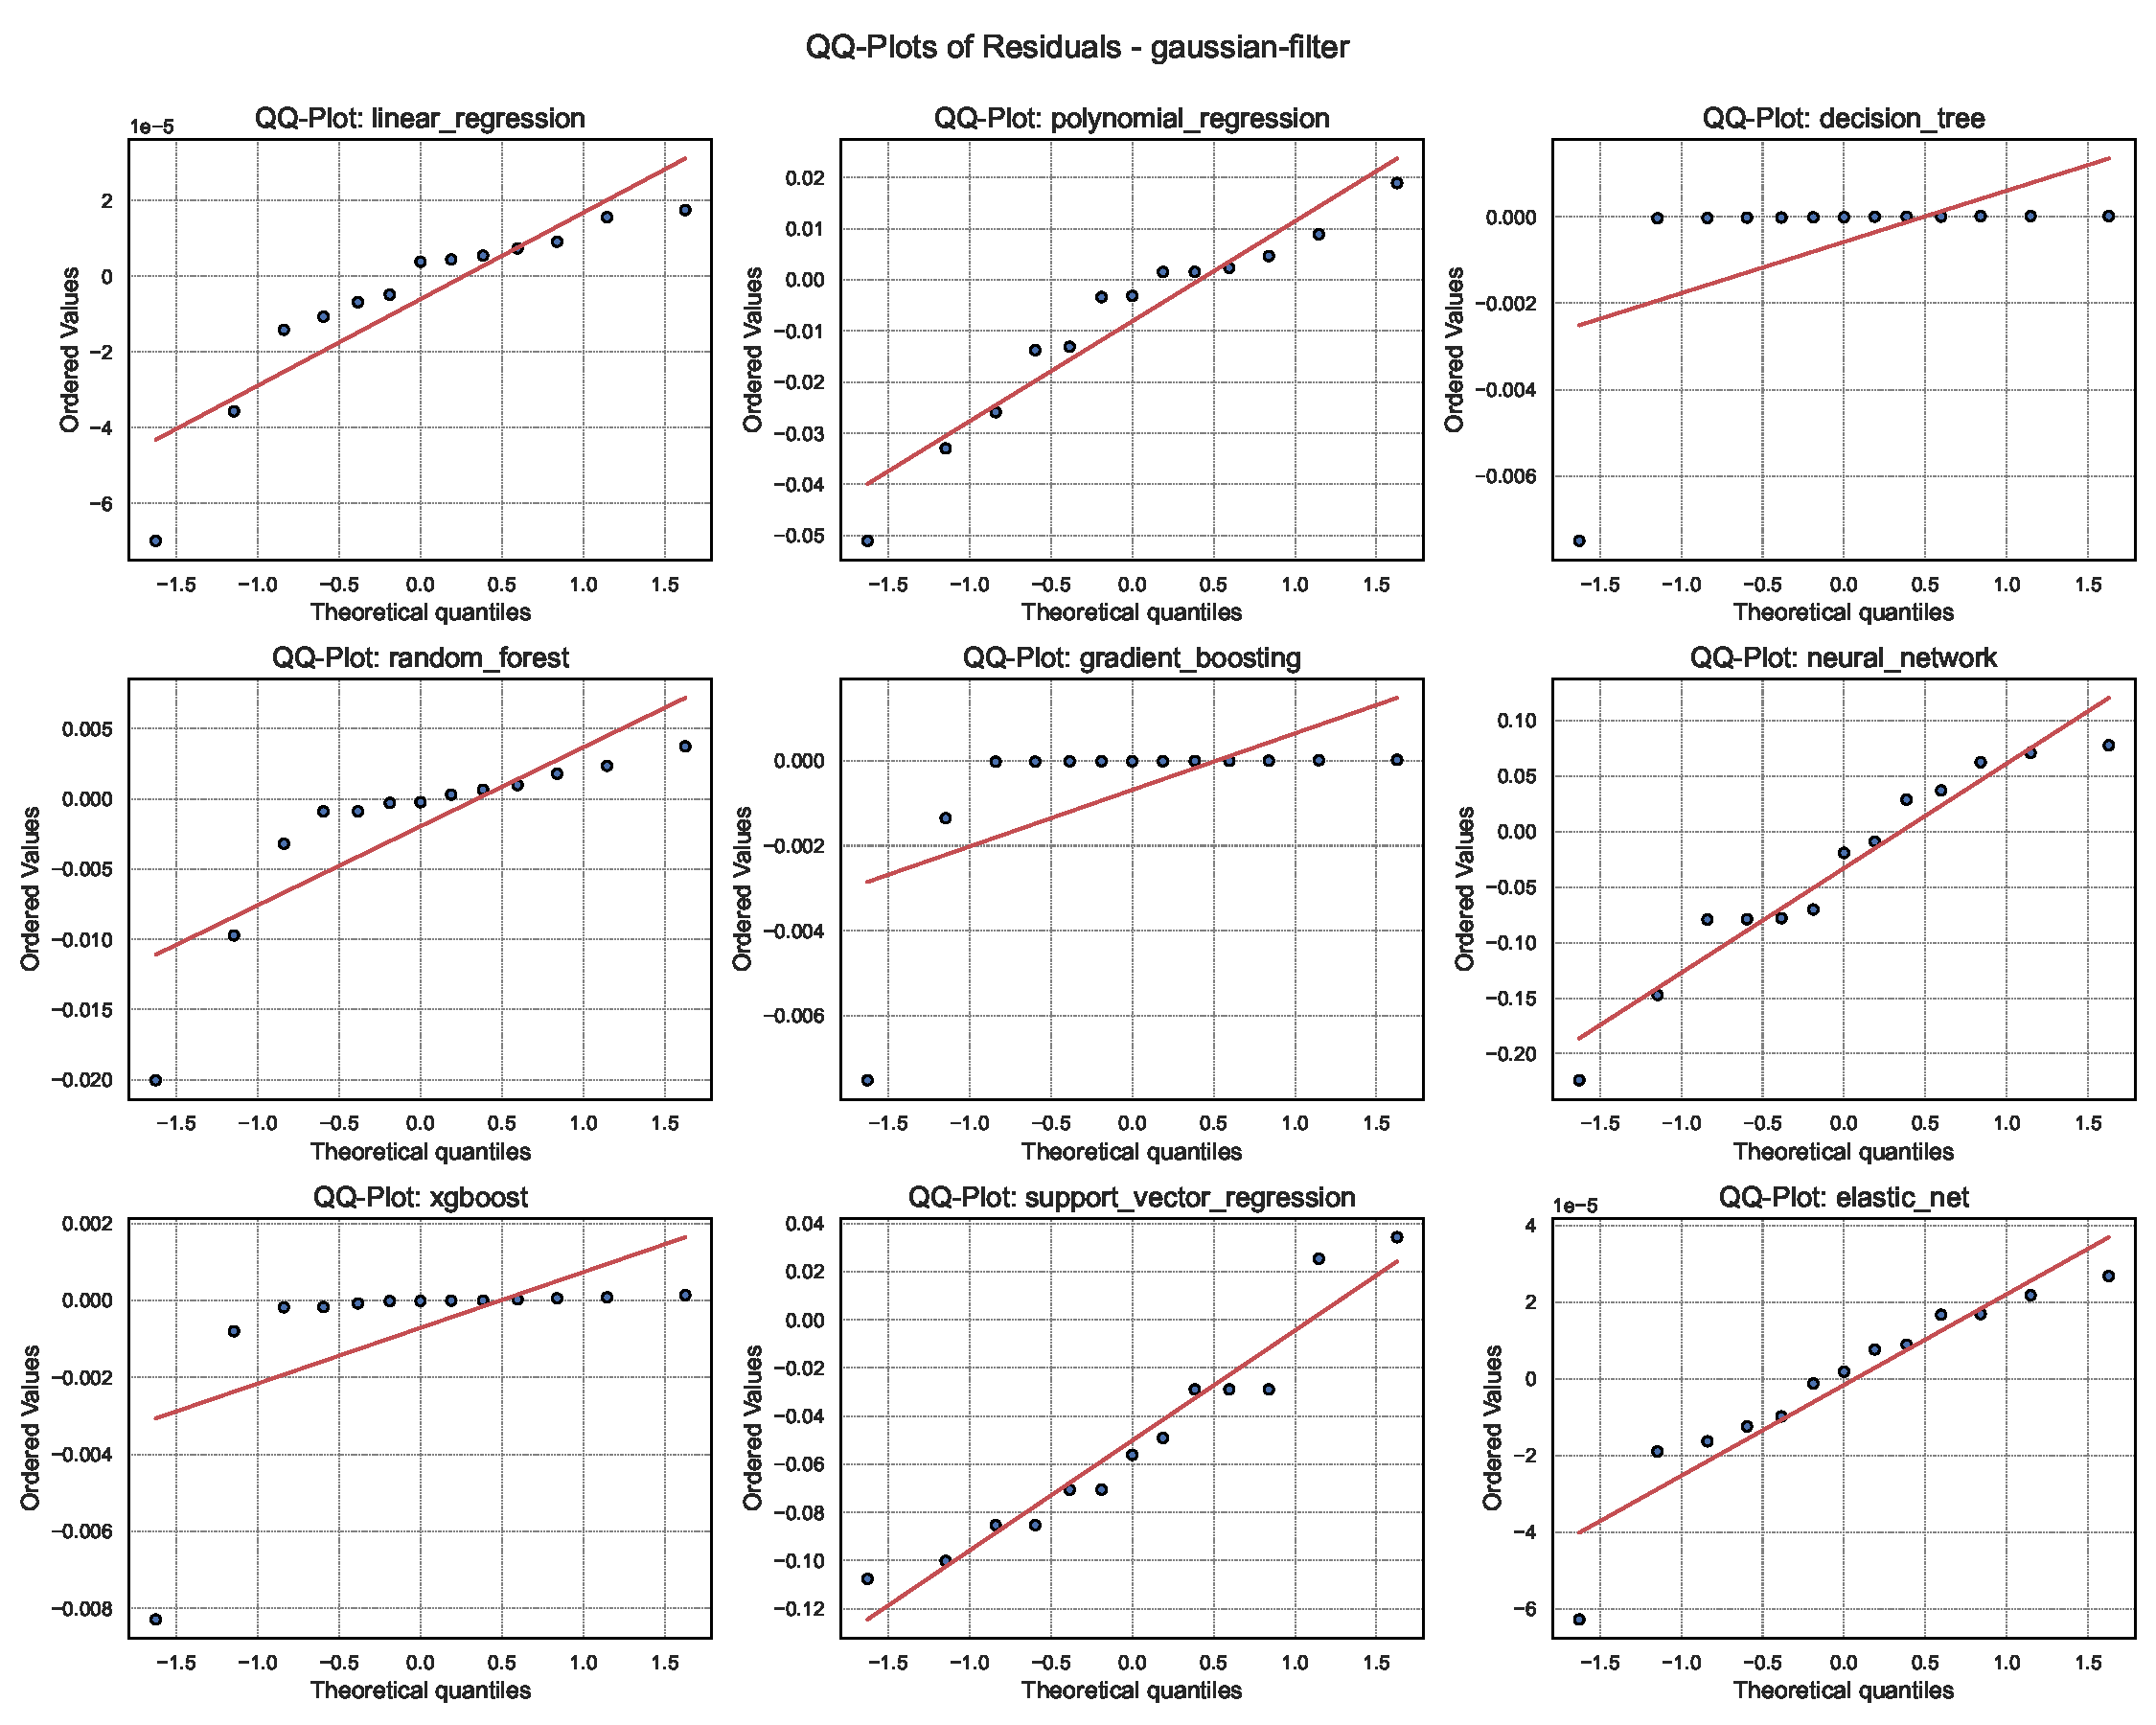
\includegraphics[width=\textwidth]{assets/images/05/residual_qq_plots_gaussian-filter}
        \caption{Gaussian Filter}
    \end{subfigure}
    \caption{\ac{QQ} plots of model residuals by operator.
        Most methods exhibit mild deviations from normality in the tails.
        Neural Network displays noticeably heavier upper-tail errors for \ac{GST3D}.
        \EB{Os rótulos ficaram muito pequenos. Será que este gráfico é necessário?}
        \label{fig:residual_qq_plots}
    }
\end{figure*}

\subsection{Performance Summary}
\label{subsec:performance-summary}

Figures~\ref{fig:performance_by_model_operators} compile \ac{RMSE}, \ac{MAE}, $R^2$, and accuracy into a single bar chart for each operator, offering a side-by-side visualization of model performance.
All charts reinforce the earlier observation that memory usage for Envelope and Gaussian Filter proves easier to capture accurately than \ac{GST3D}.
Decision Tree, Gradient Boosting, and XGBoost often yield high precision for \ac{GST3D}, whereas Neural Network and Polynomial Regression struggle with larger errors.

\begin{figure*}[htbp]
    \centering
    \begin{subfigure}[t]{0.32\textwidth}
        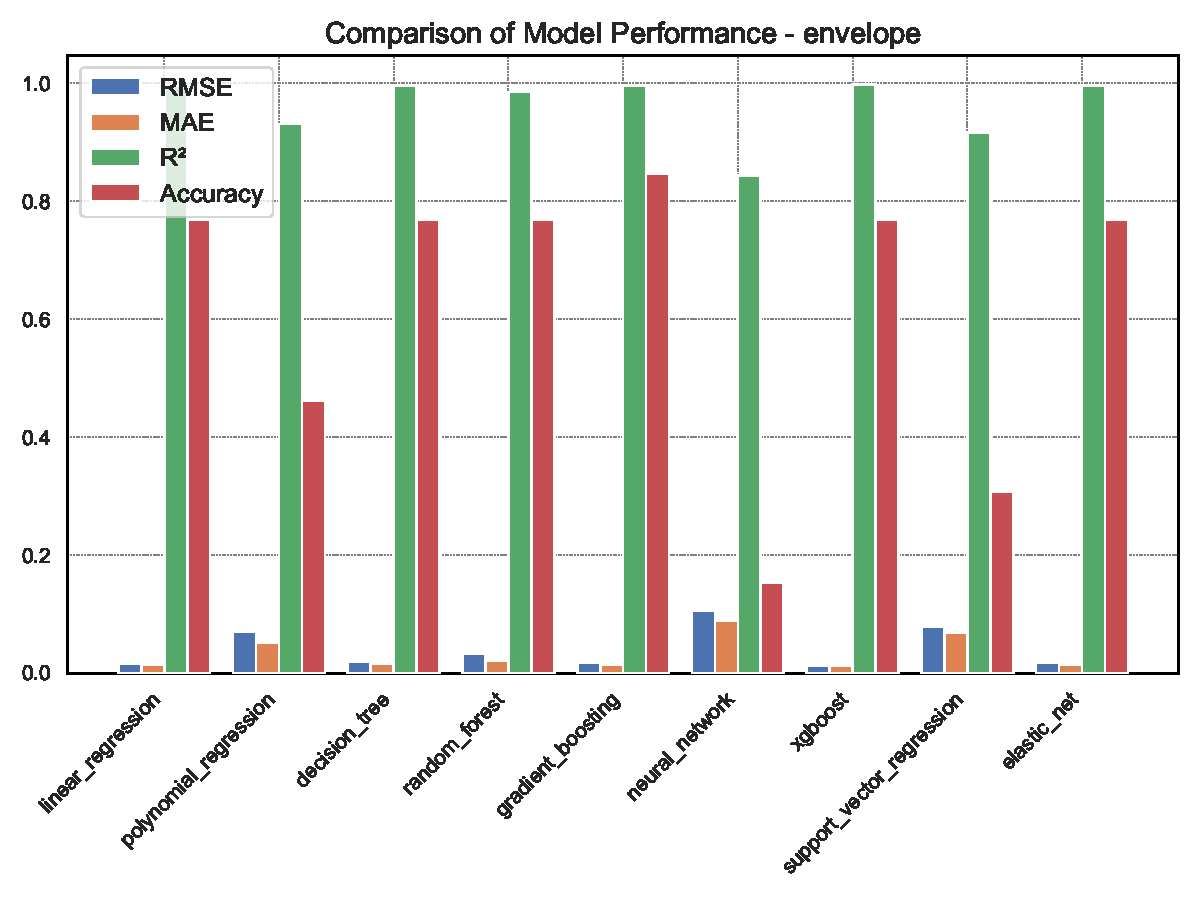
\includegraphics[width=\textwidth]{assets/images/05/performance_by_model_envelope}
        \caption{Envelope}
    \end{subfigure}
    \hfill
    \begin{subfigure}[t]{0.32\textwidth}
        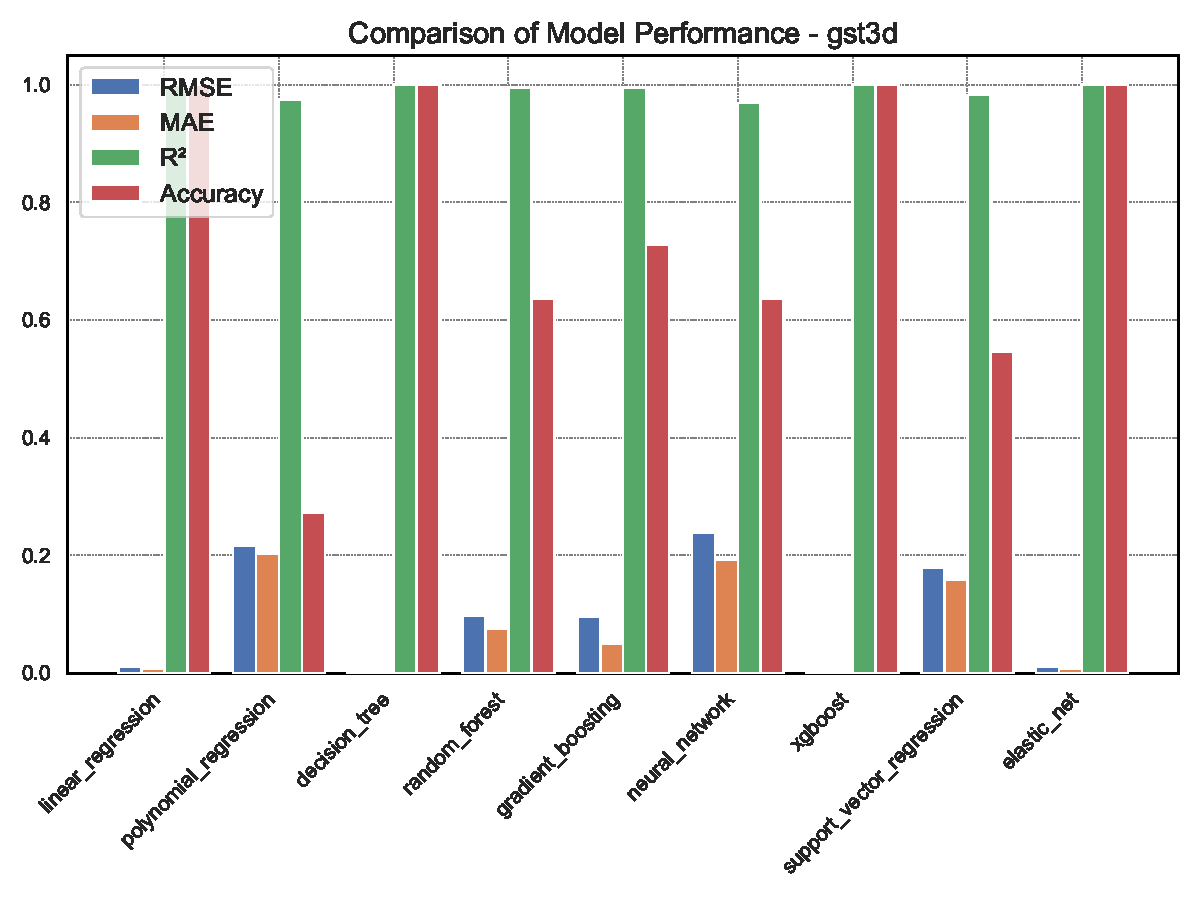
\includegraphics[width=\textwidth]{assets/images/05/performance_by_model_gst3d}
        \caption{\ac{GST3D}}
    \end{subfigure}
    \hfill
    \begin{subfigure}[t]{0.32\textwidth}
        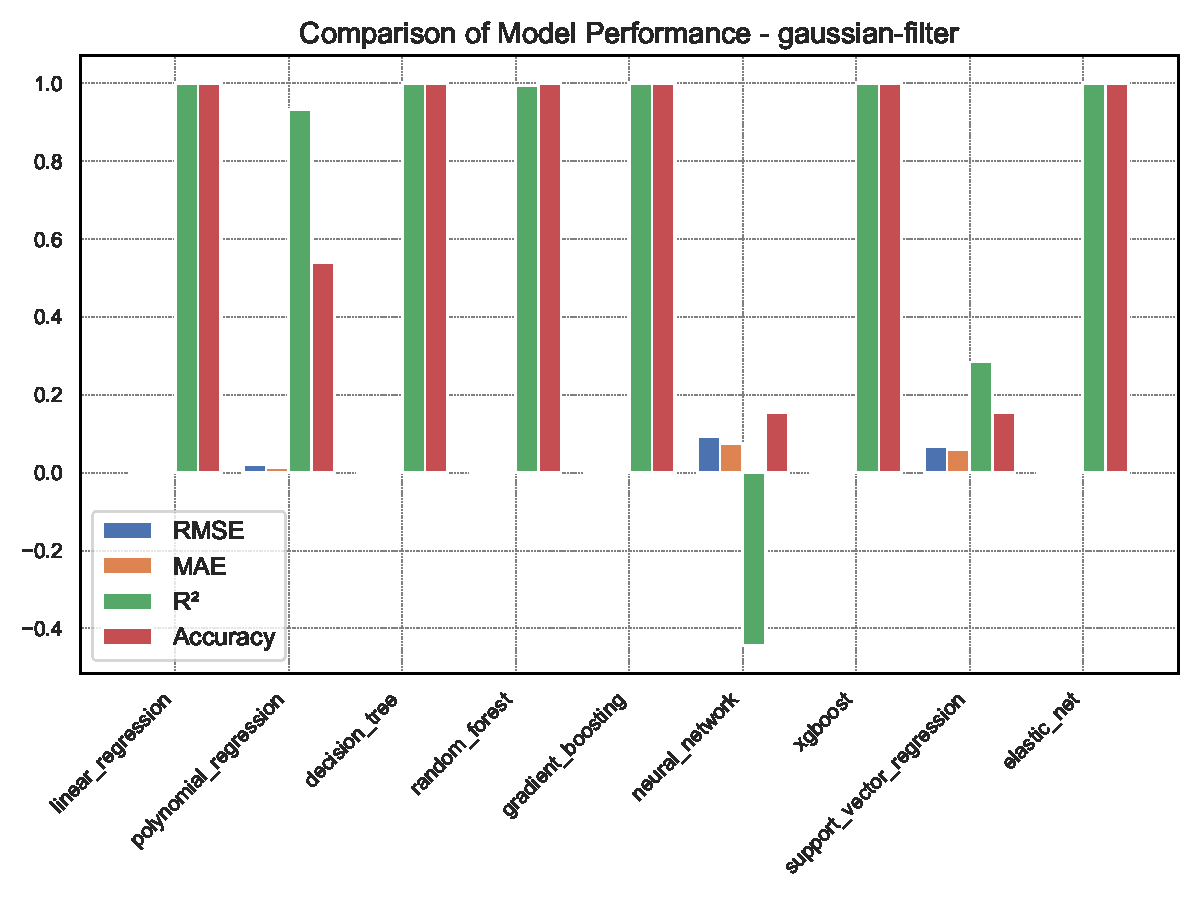
\includegraphics[width=\textwidth]{assets/images/05/performance_by_model_gaussian-filter}
        \caption{Gaussian Filter}
    \end{subfigure}
    \caption{Model metrics (\ac{RMSE}, \ac{MAE}, $R^2$, and accuracy) by operator.
        Best-in-class methods include Gradient Boosting (Envelope), Decision Tree (\ac{GST3D}), and Linear Regression (Gaussian Filter).
        \EB{Daniel, uma avaliação com valores RMSE e MAE deve levar em consideração o valor da predição - p.ex., um erro (RMSE ou MAE) de 0.1GB é pequeno em uma situação onde o valor real/predito é da ordem de dezenas ou centenas de GBs, no entanto, se o valor real/predito é da ordem de 0.1GB, o erro é bem grande.}
        \label{fig:performance_by_model_operators}
    }
\end{figure*}

In summary, the near-linear dependence of peak memory on shape parameters enables multiple models to achieve excellent accuracy and reliability.
Envelope and Gaussian Filter place fewer demands on model complexity.
\ac{GST3D} remains more challenging, though tree-based models and linear approaches still achieve high $R^2$ and low error metrics.
Neural Network stands out for relatively weaker performance in \ac{GST3D}, suggesting that the chosen architecture or hyperparameters might require further tuning for more complex operators.

All subsequent sections build on these findings to evaluate feature selection (Section~\ref{sec:pmc-results-feature-selection-experiments}) and data size reductions (Section~\ref{sec:pmc-results-data-reduction-studies}), aiming to determine whether simpler input representations or smaller datasets can maintain the strong predictive performance observed in these experiments.